\documentclass[a4paper,final]{article}
\usepackage[14pt]{extsizes}
\usepackage[T2A]{fontenc}
\usepackage[utf8]{inputenc}
\usepackage[russian]{babel}




\usepackage{amsmath}
\usepackage[left=20mm, top=20mm, right=20mm, bottom=20mm, footskip=10mm]{geometry}
\usepackage{ragged2e}
\usepackage{setspace}
\usepackage{alltt}
\usepackage{wrapfig}
\usepackage{moreverb} %листинги
\usepackage{indentfirst} % для абзацного отступа
\renewcommand\verbatimtabsize{4\relax}
\renewcommand\listingoffset{0.2em} %отступ от номеров строк
\renewcommand{\arraystretch}{1.4} % высота строки
\usepackage[font=small, singlelinecheck=false, justification=raggedleft, format=plain, labelsep=period]{caption} %заголовок таблицы
\usepackage{listings}
\usepackage{xcolor} % цвета
\usepackage{hyperref}% для гиперссылок
\usepackage{enumitem} %для перечислений
\usepackage{nccmath}
\usepackage{tikz}
\usepackage{wrapfig}
\usepackage{listings}
\usepackage{float}
\usepackage{shadow}
\usepackage{longtable}
\usepackage{multirow}
\usepackage{makecell}
\usepackage{longtable}
\usepackage{tabularx}
\usepackage{seqsplit}
\usepackage{subcaption} % Для подрисунков
\usepackage{tikz}
\usepackage{cmap}
\usetikzlibrary{shapes.geometric, arrows.meta, positioning, calc}


\hypersetup{colorlinks,
  allcolors=[RGB]{000 000 000}} %гиперссылки

\textheight=24cm
\textwidth=16cm
\oddsidemargin=0pt
\topmargin=-1.5cm
\parindent=24pt % отступ абзаца по горизонтали
\parskip=5pt % отступ абзаца по вертикали
\tolerance=2000 % терпимость
\flushbottom % выравнивание высоты
\addto\captionsrussian{\def\refname{Список использованной литературы}}
\usepackage{xcolor}

%New colors defined below
\definecolor{codegreen}{rgb}{0,0.6,0}
\definecolor{codegray}{rgb}{0.5,0.5,0.5}
\definecolor{codepurple}{rgb}{0.58,0,0.82}
\definecolor{backcolour}{rgb}{0.95,0.95,0.92}


\definecolor{apricot}{HTML}{FFF0DA}
\definecolor{mygreen}{rgb}{0,0.6,0}
\definecolor{string}{HTML}{B40000} % цвет строк в коде
\definecolor{comment}{HTML}{008000} % цвет комментариев в коде
\definecolor{keyword}{HTML}{1A00FF} % цвет ключевых слов в коде
\definecolor{morecomment}{HTML}{8000FF} % цвет include и других элементов в коде
\definecolor{captiontext}{HTML}{FFFFFF} % цвет текста заголовка в коде
\definecolor{captionbk}{HTML}{999999} % цвет фона заголовка в коде
\definecolor{bk}{HTML}{FFFFFF} % цвет фона в коде
\definecolor{frame}{HTML}{999999} % цвет рамки в коде
\definecolor{brackets}{HTML}{B40000} % цвет скобок в коде

\setlist[enumerate,itemize]{leftmargin=1.2cm}

% подгружаемые языки — подробнее в документации listings
\lstloadlanguages{C++}

\newcommand{\doublecline}[1]{\noalign{\vskip-0.5\arrayrulewidth}\cline{#1}\noalign{\vskip-0.5\arrayrulewidth}\cline{#1}}


\tikzset{
  % Терминал (прямоугольник)
  term/.style={
    rectangle, draw, rounded corners=2pt,
    minimum height=6mm, minimum width=12mm,
    inner sep=3pt, font=\ttfamily\small
  },
  % Нетерминал (угловые скобки, без рамки — курсив)
  nonterm/.style={
    rectangle, draw=none,
    minimum height=6mm,
    inner sep=2pt, font=\itshape\small
  },
  % Ключевое слово (овал — добавлено/изменено, как на оригинале)
  keyword/.style={
    ellipse, draw, fill=white,
    minimum height=6mm, minimum width=14mm,
    inner sep=3pt, font=\ttfamily\small
  },
  % Стрелка линии
  rail/.style={->, >=Stealth, thick},
  % Линия без стрелки
  wire/.style={-, thick},
}


\begin{document}
\lstset{
  inputencoding=utf8,
  language=C++, % Язык кода по умолчанию
  morekeywords={*,...}, % если хотите добавить ключевые слова, то добавляйте
  % Цвета
  keywordstyle=\color{keyword}\ttfamily\bfseries,
  %stringstyle=\color{string}\ttfamily,
  stringstyle=\ttfamily\color{red!50!brown},
  commentstyle=\color{comment}\ttfamily,
  morecomment=[l][\color{morecomment}]{\#},
  % Настройки отображения
  breaklines=true, % Перенос длинных строк
  basicstyle=\ttfamily\footnotesize, % Шрифт для отображения кода
  backgroundcolor=\color{bk}, % Цвет фона кода
  frame=lrb,xleftmargin=\fboxsep,xrightmargin=-\fboxsep, % Рамка, подогнанная к заголовку
  rulecolor=\color{frame}, % Цвет рамки
  tabsize=3, % Размер табуляции в пробелах
  % Настройка отображения номеров строк. Если не нужно, то удалите весь блок
  numbers=left, % Слева отображаются номера строк
  stepnumber=1, % Каждую строку нумеровать
  numbersep=5pt, % Отступ от кода
  numberstyle=\small\color{black}, % Стиль написания номеров строк
  % Для отображения русского языка
  extendedchars=true,
  literate=
  {→}{{\ensuremath{\rightarrow}}}1
  {ε}{{\ensuremath{\varepsilon}}}1
  {á}{{\'a}}1  {é}{{\'e}}1  {í}{{\'i}}1  {ó}{{\'o}}1  {ú}{{\'u}}1
  {Á}{{\'A}}1  {É}{{\'E}}1  {Í}{{\'I}}1  {Ó}{{\'O}}1  {Ú}{{\'U}}1
  {ñ}{{\~n}}1  {Ñ}{{\~N}}1  {¿}{{{\textquestiondown}}}1  {¡}{{{\textexclamdown}}}1
  {Ö}{ {\''O} }1
  {~}{ {\textasciitilde} }1
  {а}{ {\selectfont\char224} }1
  {б}{ {\selectfont\char225} }1
  {в}{ {\selectfont\char226} }1
  {г}{ {\selectfont\char227} }1
  {д}{ {\selectfont\char228} }1
  {е}{ {\selectfont\char229} }1
  {ё}{ {\''e} }1
  {ж}{ {\selectfont\char230} }1
  {з}{ {\selectfont\char231} }1
  {и}{ {\selectfont\char232} }1
  {й}{ {\selectfont\char233} }1
  {к}{ {\selectfont\char234} }1
  {л}{ {\selectfont\char235} }1
  {м}{ {\selectfont\char236} }1
  {н}{ {\selectfont\char237} }1
  {о}{ {\selectfont\char238} }1
  {п}{ {\selectfont\char239} }1
  {р}{ {\selectfont\char240} }1
  {с}{ {\selectfont\char241} }1
  {т}{ {\selectfont\char242} }1
  {у}{ {\selectfont\char243} }1
  {ф}{ {\selectfont\char244} }1
  {х}{ {\selectfont\char245} }1
  {ц}{ {\selectfont\char246} }1
  {ч}{ {\selectfont\char247} }1
  {ш}{ {\selectfont\char248} }1
  {щ}{ {\selectfont\char249} }1
  {ъ}{ {\selectfont\char250} }1
  {ы}{ {\selectfont\char251} }1
  {ь}{ {\selectfont\char252} }1
  {э}{ {\selectfont\char253} }1
  {ю}{ {\selectfont\char254} }1
  {я}{ {\selectfont\char255} }1
  {А}{ {\selectfont\char192} }1
  {Б}{ {\selectfont\char193} }1
  {В}{ {\selectfont\char194} }1
  {Г}{ {\selectfont\char195} }1
  {Д}{ {\selectfont\char196} }1
  {Е}{ {\selectfont\char197} }1
  {Ё}{ {\''E} }1
  {Ж}{ {\selectfont\char198} }1
  {З}{ {\selectfont\char199} }1
  {И}{ {\selectfont\char200} }1
  {Й}{ {\selectfont\char201} }1
  {К}{ {\selectfont\char202} }1
  {Л}{ {\selectfont\char203} }1
  {М}{ {\selectfont\char204} }1
  {Н}{ {\selectfont\char205} }1
  {О}{ {\selectfont\char206} }1
  {П}{ {\selectfont\char207} }1
  {Р}{ {\selectfont\char208} }1
  {С}{ {\selectfont\char209} }1
  {Т}{ {\selectfont\char210} }1
  {У}{ {\selectfont\char211} }1
  {Ф}{ {\selectfont\char212} }1
  {Х}{ {\selectfont\char213} }1
  {Ц}{ {\selectfont\char214} }1
  {Ч}{ {\selectfont\char215} }1
  {Ш}{ {\selectfont\char216} }1
  {Щ}{ {\selectfont\char217} }1
  {Ъ}{ {\selectfont\char218} }1
  {Ы}{ {\selectfont\char219} }1
  {Ь}{ {\selectfont\char220} }1
  {Э}{ {\selectfont\char221} }1
  {Ю}{ {\selectfont\char222} }1
  {Я}{ {\selectfont\char223} }1
  {\{}{ { {\color{brackets}\{} } }1 % Цвет скобок {
  {\} }{ { {\color{brackets}\} } } }1 % Цвет скобок }
}


\thispagestyle{empty}
\begin{center}
\hfill \break
\hfill \break
\normalsize{МИНИСТЕРСТВО НАУКИ И ВЫСШЕГО ОБРАЗОВАНИЯ РОССИЙСКОЙ ФЕДЕРАЦИИ\\
 федеральное государственное автономное образовательное учреждение высшего образования «Санкт-Петербургский политехнический университет Петра Великого»\\[10pt]}
\normalsize{Институт компьютерных наук и кибербезопасности}\\[10pt] 
\normalsize{Высшая школа технологий искусственного интеллекта}\\[10pt] 
\normalsize{Направление: 02.03.01 <<Математика и компьютерные науки>>}\\
\vspace{50pt}
{\large Математическая логика и теория формальных языков\\
Отчёт о выполнении лабораторной работы №4 \\[1em]
<<Доработка компилятора языка MiLan>>}
\end{center}
 \vspace{70pt}
\small{ 
\begin{tabular}{lrrl}
\!\!\!Студент, & \hspace{2cm} & & \\
\!\!\!группа 5130201/30102 & \hspace{2cm} & \underline{\hspace{3cm}} & Путята М. А.  \\\\
\!\!\!Преподаватель & \hspace{2cm} & \underline{\hspace{3cm}} &  Востров А. В. \\\\
&&\hspace{5cm}
\end{tabular}
\begin{flushright}
<<\underline{\hspace{1cm}}>>\underline{\hspace{2.5cm}} 2026 г.
\end{flushright}
}

\hfill \break
\begin{center} \small{Санкт-Петербург, 2026} \end{center}


\newpage
\tableofcontents
\newpage


\section*{Введение}
\addcontentsline{toc}{section}{Введение}
Лабораторная работа №4 заключается в доработке компилятора и виртуальной машины языка MiLan. В рамках данного варианта реализована поддержка работы со строками.

В данной лабораторной работе необходимо доработать компилятор языка MiLan согласно заданному варианту.

\textbf{Вариант 7}: Оператор выбора
\begin{verbatim}
    switch(<выражение>)
    begin
        case <значение 1>: <список операторов> break;
        case <значение 2>: <список операторов> break;
        ...
        default: <список операторов>
    endcase
\end{verbatim}

Также дополнительно к основному варианту будут реализованы следующие доработки компилятора:
\begin{itemize}
    \item Оператор цикла
\begin{verbatim}
    for(<инициализация>; <условие>; <выражение>) do
        <список операторов>
    od
\end{verbatim}
    \item Булевы константы, переменные и операции (\&, \&\&, |, || !).
    \item Одномерные массивы и операции над ними (заполнение, поиск элемента, длина, замена элемента, реверс, изменение размера, сортировка, взятие элемента по индексу, взятие среза).
    \item Двумерные массивы и операции над ними (заполнение, поиск элемента, длина, замена элемента, реверс, изменение размера, сортировка, превращение в вектор, транспонирование, взятие элемента по индексу, взятие среза)
    \item Поэлементные арифметические операции над одномерными и двумерными массивами.
    \item Все виды комментариев (однострочные и многострочные).
    \item Перемножение двумерных массивов по правилам Шимбелла -- \texttt{shimb(a, b, 1/0)}
\end{itemize}

\newpage
\section*{Постановка задачи}
\addcontentsline{toc}{section}{Постановка задачи}
Для выполнения поставленной задачи необходимо:
\begin{enumerate}
    \item Проанализировать существующие языки программирования (С++, Ruby, JavaScript), на которых будет основан синтаксис доработок компилятора.
    \item Изучить работу булевых операций в Java.
    \item Выбрать типы операторов для одномерных и двумерных массивов (мутирующие или иммутабельные).
    \item Создать новую синтаксическую диаграмму для лексического анализатора.
    \item Расширить формальную грамматику языка MiLan в БНФ-нотации.
    \item Построить синтаксические диаграммы расширенного языка MiLan.
    \item Реализовать поддержку новых типов данных и операторов в компиляторе.
\end{enumerate}

\newpage
\section{Математическое описание}

\subsection{Язык MiLan}
Язык Милан --- простой учебный язык программирования, в котором поддерживаются только целочисленные константы и идентификаторы, операторы присваивания, арифметические действия и сравнения. Также данный язык позволяет использовать управляющие конструкции (\texttt{if ... then ... else ... fi}, \texttt{while ... do ... od}, \texttt{begin ... end}) и IO-команды (\texttt{read}, \texttt{write}).

Программа написанная на языке Milan пишется между ключевыми словами \texttt{begin} и \texttt{end} и состоит из последовательности операторов и управляющих конструкций. Все операторы отделяются друг от друга с помощью точки с запятой, а после последнего оператора в блоке она не ставится. При компиляции программы не учитывается регистр символов.


\subsection{Лексический анализатор языка Milan}
Лексический анализатор проводит лексический анализ (первый этап трансляции), выделяя лексемы входного языка -- минимальные единицы языка, которые имеют смысл. В естественном языке лексемами являются слова, а в языке программирования -- идентификаторы, служебные символы, константы, операторы и т.д..

Так как к компилятору будет применено большое количество доработок было решено переписать лексический анализатор с нуля, реализовав его с помощью конечного автомата. Данное решение позволяет увеличить скорость обработки исходного кода программы.

Лексический анализатор реализуется с помощью конечного автомата, преобразующего входную цепочку символов в последовательность пар <Тип лексемы, Значение>.

Если заданы:
\begin{itemize}
    \item $\displaystyle \Sigma$ = \{\textbackslash t, \textbackslash n, ''\_'', (, ), [, ], \{, \}, *, +, -, /, ., :, ;, =, !, <, >, |, \& \} $\cup$ \{0, \dots, 9]\} $\cup$ \{A, \dots, Z\} $\cup$ \{ a, \dots, z \} -- входной алфавит;
    \item $\displaystyle T$ = \{ Div,
Id, Arith, LBracket, RBracket, LCurly, RCurly, LSquare, RSquare, Assign, Semicolon, Comma, Var, Logical, Cmp, Keyword, Func, Comment, MultiComment \} -- множество типов лексем.
    \item $D$ = \{ begin, end, if, then, else, fi, while, do, od, for, switch, case, default, endcase, break, int, bool, true, false, read, write, find, len, reverse, resize, replace, sorted, tovector, trans, shimb, fill, :=, =, ;, ,, :, !, \&, \&\&, |, ||, =, !=, <, <=, >, >=, +, -, *, /, (, ), ''\{'', ''\}'', [, ], \} $\cup ~D_{id} \cup D_{var}$ -- множество допустимых значений лексем, где
    \begin{itemize}
        \item $D_{id} = \left\{s \in \Sigma_{id}^+~~ \middle|~~\begin{array}{l}
            |s| \in [1, 63], \\
            s[0] \in \{A, \dots, Z\} \cup \{ a, \dots, z \}, \\
            \forall i \in [1, 63]: s[i] \in \Sigma_{id}
        \end{array}
        \right\}$,\\[1em]
        $\Sigma_{id} = \{A, \dots, Z\} \cup \{ a, \dots, z \} \cup \{ 0, \dots, 9 \}$
        \item $D_{const} = \left\{s \in \Sigma_{const}^+~~ \middle|~~\begin{array}{l}
            |s| \in [1, 10],\\
            |s| > 1 \rightarrow s[0] \neq 0
        \end{array}
        \right\}$\\[1em]
        $\Sigma_{const} = \{ 0, \dots, 9 \}$
    \end{itemize}
\end{itemize}
То лексический анализатор будет реализовывать отображение $\displaystyle \Sigma^* \longrightarrow (T \times D)^*$, где
\begin{itemize}
    \item $\displaystyle \Sigma^*$ -- замыкание алфавита входного языка;
    \item $(T \times D)^*$ -- множество пар <Тип лексемы, Значение>.
\end{itemize}

Для представления поведения конечного автомата (в данном случае лексического анализатора) можно использовать синтаксическую диаграмму, получаемую с помощью преобразования КА. Далее на рисунках 1 - 3 представлена синтаксическая диаграмма для лексического анализатора, разработанного для языка MiLan.

\begin{figure}[H]
    \centering
    
\includegraphics[width=0.9\linewidth]{image1.png}
    \caption{\centering Синтаксическая диаграмма лексического анализатора. Часть 1}
\end{figure}

\begin{figure}[H]
    \centering
    
\includegraphics[width=0.8\linewidth]{image2.png}
    \caption{\centering Синтаксическая диаграмма лексического анализатора. Часть 2}
\end{figure}

\begin{figure}[H]
    \centering
    
\includegraphics[width=0.9\linewidth]{image3.png}
    \caption{\centering Синтаксическая диаграмма лексического анализатора. Часть 3}
\end{figure}

Действия используемые в синтаксической диаграмме:
\begin{itemize}
    \item y1 -- сдвиг каретки;
    \item y2 -- запись текущего символа в буфер;
    \item y3 -- очистка буфера;
    \item y\_Div -- выдать лексему <arith, />;
    \item y\_Id -- выдать лексему <Id, значение>;
    \item y\_Plus -- выдать лексему <arith, +>;
    \item y\_Diff -- выдать лексему <arith, ->;
    \item y\_Mult -- выдать лексему <arith, *>;
    \item y\_LBracket -- выдать лексему <LBracket, (>;
    \item y\_RBracket -- выдать лексему <RBracket, )>;
    \item y\_LCurly -- выдать лексему <LCurly, \{>;
    \item y\_RCurly -- выдать лексему <RCurly, \}>;
    \item y\_LSquare -- выдать лексему <LSquare, [>;
    \item y\_RSquare -- выдать лексему <RSquare, ]>;
    \item y\_Assign -- выдать лексему <Assign, :=>;
    \item y\_Semicolon -- выдать лексему <Semicolon, ;>;
    \item y\_Comma -- выдать лексему <Comma, ,>;
    \item y\_Var -- выдать лексему <Keyword, var>;
    \item y\_ShortAnd -- выдать лексему <Logic, \&\&>;
    \item y\_FullAnd -- выдать лексему <Logic, \&>;
    \item y\_ShortOr -- выдать лексему <Logic, ||>;
    \item y\_FullOr -- выдать лексему <Logic, |>;
    \item y\_Equal -- выдать лексему <Cmp, =>;
    \item y\_NotEqual -- выдать лексему <Cmp, !=>;
    \item y\_Not -- выдать лексему <Logic, not>;
    \item y\_LessEqual -- выдать лексему <Cmp, <= >;
    \item y\_Less -- выдать лексему <Cmp, < >;
    \item y\_GreaterEqual -- выдать лексему <Cmp, >= >;
    \item y\_Greater -- выдать лексему <Cmp, > >;
    \item y\_Begin -- выдать лексему <Keyword, begin>;
    \item y\_Break -- выдать лексему <Keyword, break>;
    \item y\_Bool -- выдать лексему <Keyword, bool>;
    \item y\_Case -- выдать лексему <Keyword, case>;
    \item y\_Colon -- выдать лексему <Colon, :>;
    \item y\_Default -- выдать лексему <Keyword, default>;
    \item y\_Do -- выдать лексему <Keyword, do>;
    \item y\_End -- выдать лексему <Keyword, end>;
    \item y\_EndCase -- выдать лексему <Keyword, endcase>;
    \item y\_Else -- выдать лексему <Keyword, else>;
    \item y\_For -- выдать лексему <Keyword, for>;
    \item y\_False -- выдать лексему <Var, 0>;
    \item y\_Find -- выдать лексему <Func, find>;
    \item y\_Fi -- выдать лексему <Keyword, fi>;
    \item y\_Int -- выдать лексему <Keyword, int>;
    \item y\_If -- выдать лексему <Keyword, if>;
    \item y\_Len -- выдать лексему <Func, len>;
    \item y\_Od -- выдать лексему <Keyword, od>;
    \item y\_Replace -- выдать лексему <Func, replace>;
    \item y\_Reverse -- выдать лексему <Func, reverse>;
    \item y\_Resize -- выдать лексему <Func, resize>;
    \item y\_Read -- выдать лексему <Keyword, read>;
    \item y\_Switch -- выдать лексему <Keyword, switch>;
    \item y\_Shimb -- выдать лексему <Func, Shimb>;
    \item y\_Sorted -- выдать лексему <Func, sorted>;
    \item y\_True -- выдать лексему <Var, 1>;
    \item y\_Then -- выдать лексему <Keyword, then>;
    \item y\_ToVector -- выдать лексему <Func, tovector>;
    \item y\_Trans -- выдать лексему <Func, trans>;
    \item y\_While -- выдать лексему <Keyword, while>;
    \item y\_Write -- выдать лексему <Keyword, write>;
    \item y\_Comment -- выдать лексему <Comment, значение>;
    \item y\_MultiComment -- выдать лексему <MultiComment, значение>;
    \item y\_Fill -- выдать лексему <Func, fill>;
\end{itemize}


\subsection{Грамматика языка MiLan}
Синтаксис языка MiLan определяется контекстно-свободной грамматикой, которая в иерархии Хомского относится к типу 2. Её ключевое свойство заключается в том, что левая часть любого правила вывода содержит ровно один нетерминальный символ (правила вывода имеют вид $A \to \gamma$). Все синтаксические конструкции MiLan подчиняются этому условию, поэтому его грамматика является контекстно-свободной.

Для разбора последовательностей лексем используется нисходящий синтаксический анализатор, реализованный методом рекурсивного спуска. Данный подход требует, чтобы грамматика обладала свойством LL(1): это позволяет строить для каждого нетерминала однозначные синтаксические диаграммы, где выбор следующей ветви определяется детерминированно по одной следующей лексеме. Свойство LL(1) гарантирует, что для корректного применения правила вывода достаточно знать текущий контекст анализа и первый ещё не обработанный терминал входной строки.

Контекстно-свободная грамматика задаётся как четверка объектов $G = (T, N, S, R)$, где:
\begin{itemize}
    \item $T$ --- конечное множество терминальных символов: T = \{begin, end, if, then, else, fi, while, do, od, for, switch, case, default, endcase, break, int, bool, true, false, read, write, find, len, reverse, resize, replace, sorted, tovector, trans, shimb, fill, :=, =, ;, ,, :, !, \&, \&\&, |, ||, =, !=, <, <=, >, >=, +, -, *, /, (, ), ''\{'', ''\}'', [, ], identifier, integer\}.
    \item $N$ --- конечное множество нетерминальных символов: N = \{<Program>, <DeclList>, <Decl>, <Type>, <IdentList>, <IdentInit>, <ArrayInit>, <MatrixInit>, <MatrixRow>, <StmtList>, <Stmt>, <AssignStmt>, <IfStmt>, <WhileStmt>, <ForStmt>, <SwitchStmt>, <CaseList>, <Case>, <DefaultOpt>, <ForInit>, <ForStep>, <WriteArg>, <Expr>, <BoolExpr>, <BoolTerm>, <BoolFactor>, <BoolPrimary>, <ArithExpr>, <Term>, <Factor>, <Primary>, <CmpOp>, <ArrayExpr>, <ArrayFuncExpr>, <IndexExpr>, <SliceExpr>, <ArgList>\}.
    \item $S \in N$ --- начальный нетерминал: S = <program>.
    \item $R$ --- конечное множество правил вывода вида $A \to \gamma$, где $A \in N$, $\gamma \in (T \cup N)^*$. Множество $R$ задаётся следующими правилами вывода (где $|$ обозначает альтернативу, а $[\cdot]$ --- необязательный элемент и $\{\cdot\}$ --- повторение 0 или более раз):
    \begin{itemize}
\item <program>      → begin <DeclSeq> <StmtSeq> end
\item <DeclSeq>      → <type> <ident-list> ; <DeclSeq> | \ensuremath{\varepsilon}
\item <StmtSeq>      → <stmt> ; <StmtSeq> | <stmt> <StmtSeq> | \ensuremath{\varepsilon}
\item <type>         → int | bool
\item <ident-list>   → <ident-init> | <ident-init> , <ident-list>
\item <ident-init>   → <id> := <expr>
                \\| <id>
                \\| <id> [ <integer> ] := <array-expr>
                \\| <id> [ <integer> ] = <array-expr>
                \\| <id> [ <integer> ]
                \\| <id> [ <integer> ] [ <integer> ] := <array-expr>
                \\| <id> [ <integer> ] [ <integer> ] = <array-expr>
                \\| <id> [ <integer> ] [ <integer> ]
\item <stmt>      <id> <assign-tail>
                \\| if <expr> then <StmtSeq> fi
                \\| if <expr> then <StmtSeq> else <StmtSeq> fi
                \\| while <expr> do <StmtSeq> od
                \\| for ( <ForInitOpt> ; <expr> ; <ForStepOpt> ) do <StmtSeq> od
                \\| switch ( <expr> ) begin <CaseSeq> <DefaultOpt> endcase
                \\| break
                \\| write ( <write-arg> )
                \\| read ( <id> )
                \\| read ( <id> [ <expr> ] )
                \\| read ( <id> [ <expr> ] [ <expr> ] )
                \\| <builtin-call>
\item <ForInitOpt>   → <for-init> | \ensuremath{\varepsilon}
\item <ForStepOpt>   → <for-step> | \ensuremath{\varepsilon}
\item <CaseSeq>      → <Case> <CaseSeq> | \ensuremath{\varepsilon}
\item <Case>         → case <expr> : <StmtSeq> break ; \\| case <expr> : <StmtSeq>
\item <DefaultOpt>   → default : <StmtSeq> | \ensuremath{\varepsilon}
\item <assign-tail>  → := <expr>
                \\| := <array-expr>
                \\| [ <expr> ] := <expr>
                \\| [ <expr> ] [ <expr> ] := <expr>
                \\| [ <integer> ] := <array-expr>
\item <for-init>     → <type> <id> := <expr> | <id> := <expr>
\item <for-step>     → <id> := <expr>
\item <write-arg>    → <expr> \\| <array-expr> \\| <id> [ <integer> ] \\| <id> [ <integer> : <integer> ]
\item <builtin-call> → find ( <array-expr> , <expr> )
                \\| find ( <array-expr> , <array-expr> )
                \\| len ( <len-arg> )
                \\| reverse ( <array-expr> )
                \\| sorted ( <array-expr> )
                \\| sorted ( <array-expr> , <integer> )
                \\| trans ( <array-expr> )
                \\| tovector ( <id> )
                \\| shimb ( <array-expr> , <array-expr> , <bool-val> )
                \\| resize ( <array-expr> , <integer> , <expr> )
                \\| resize ( <array-expr> , <integer> , <array-expr> )
                \\| replace ( <array-expr> , <expr> , <expr> )
                \\| replace ( <array-expr> , <expr> , <array-expr> )
                \\| replace ( <array-expr> , <array-expr> , <expr> )
                \\| replace ( <array-expr> , <array-expr> , <array-expr> )
                \\| fill ( <id> , <expr> )
                \\| fill ( <id> [ <integer> ] , <expr> )
\item <expr>         → <bool-term> | <bool-term> || <expr> \\| <bool-term> | <expr>
\item <bool-term>    → <bool-factor> \\| <bool-factor> \&\& <bool-term> \\| <bool-factor> \& <bool-term>
\item <bool-factor>  → ! <bool-primary> | <bool-primary>
\item <bool-primary> → true | false
                \\| <arith-expr> <=> <arith-expr>
                \\| <arith-expr> != <arith-expr>
                \\| <arith-expr> < <arith-expr>
                \\| <arith-expr> <= <arith-expr>
                \\| <arith-expr> > <arith-expr>
                \\| <arith-expr> >= <arith-expr>
\item <arith-expr>   → <term> \\| <term> + <arith-expr> \\| <term> - <arith-expr>
\item <term>         → <factor> \\| <factor> * <term> \\| <factor> / <term>
\item <factor>       → - <primary> \\| ( int ) <primary> \\| <primary>
\item <primary>      → <integer> | true | false
                \\| <id>
                \\| <id> [ <expr> ]
                \\| <id> [ <expr> ] [ <expr> ]
                \\| <id> [ <integer> : <integer> ]
                \\| ( <expr> )
                \\| read ()
                \\| <builtin-call>
\item <array-expr>   → { <elem-list> } \\| { <row-list> }
                \\| <id> \\| <id> [ <integer> ] \\| <id> [ <integer> : <integer> ]
                \\| sorted ( <array-expr> ) \\| sorted ( <array-expr> , <integer> )
                \\| trans ( <array-expr> ) \\| tovector ( <id> )
                \\| shimb ( <array-expr> , <array-expr> , <bool-val> )
                \\| resize ( <array-expr> , <integer> , <expr> ) \\| resize ( <array-expr> , <integer> , <array-expr> )
                \\| replace ( <array-expr> , <expr> , <expr> ) \\| replace ( <array-expr> , <expr> , <array-expr> )
                \\| replace ( <array-expr> , <array-expr> , <expr> ) \\| replace ( <array-expr> , <array-expr> , <array-expr> )
\item <elem-list>    → <expr> \\| <expr> , <elem-list>
\item <row-list>     → { <elem-list> } \\| { <elem-list> } , <row-list>
\item <len-arg>      → <id> \\| <id> [ <expr> ] \\| <id> [ <integer> : <integer> ] \\| <array-expr>
\item <bool-val>     → 0 \\| 1 \\| true \\| false
\item <id>           → <letter> <IdTail>
\item <IdTail>       → <letter> <IdTail> \\| <digit> <IdTail> \\| \ensuremath{\varepsilon}
\item <integer>      → <digit> <IntTail>
\item <IntTail>      → <digit> <IntTail> \\| \ensuremath{\varepsilon}
\item <digit>        → 0 | 1 | 2 | 3 | 4 | 5 | 6 | 7 | 8 | 9
\item <letter>       → a | b | ... | z \\| A | B | ... | Z
    \end{itemize}
\end{itemize}

\subsection{Описание операторов}
В течении выполнения данной лабораторной работы были добавлены следующие операторы:
\begin{itemize}
    \item len(array/matrix) -- возвращает длину заданного одномерного или двумерного массива.
    \item replace(array/matrix, i, j) -- изменяет заданный одномерный или двумерный массив, заменяя все вхождения элемента i на элемент j.
    \item reverse(array/matrix) -- изменяет заданный одномерный или двумерный массив, меняя порядок следования жэлементов на обратный.
    \item resize(array/matrix, n, i) -- изменяет размер заданного одномерного или двумерного массив, если n больше текущей длины, то массив обрезается, иначе добавляется $n - l$ элементов i в конец массива, где $l$ -- длина массива.
    \item sorted(array) -- сортирует элементы заданного одномерного массива.
    \item sorted(matrix, i) -- сортируется элементы двумерного массива по значениям их i-ых элементов.
    \item tovector(matrix) -- возвращает плоский вектор, образованный из элементов заданного двумерного массива.
    \item trans(matrix) -- производит транспонирование заданного двумерного массива.
    \item fill(array/matrix, i) -- заполняет заданный одномерный или двумерный массив элементами i.
    \item find(array/matrix, i) -- возвращает позицию элемента i в заданном одномерном или двумерном массиве.
    \item shimb(array1, array2, 1/0) -- возвращает двумерный массив, являющийся результатом перемножения заданных двумерных массивов по правилам Шимбелла.    
\end{itemize}

\subsection{Грамматика в БНФ}
Расширенная грамматика языка MiLan с поддержкой новых конструкций и операторов приведена ниже.

\begin{lstlisting}[language=TeX,basicstyle=\ttfamily\footnotesize]
<program> ::= "begin" {<type> <ident-list> ";"} {<stmt> [";"]} "end"

<type> ::= "int" | "bool"

<ident-list> ::= <ident-init> {"," <ident-init>}

<ident-init> ::= <id> [":=" <expr>]
               | <id> "[" <integer> "]" [(":=") <array-expr>]
               | <id> "[" <integer> "]" "[" <integer> "]" [(":=") <array-expr>]

<stmt> ::= <id> <assign-tail>
         | "if" <expr> "then" {<stmt> [";"]} ["else" {<stmt> [";"]}] "fi"
         | "while" <expr> "do" {<stmt> [";"]} "od"
         | "for" "(" [<for-init>] ";" <expr> ";" [<for-step>] ")" "do" {<stmt> [";"]} "od"
         | "switch" "(" <expr> ")" "begin" {"case" <expr> ":" {<stmt> [";"]} ["break"]} ["default" ":" {<stmt> [";"]}] "endcase"
         | "break"
         | "write" "(" <write-arg> ")"
         | "read" "(" <id> ["[" <expr> "]" ["[" <expr> "]"]] ")"
         | <builtin-call>

<assign-tail> ::= ":=" <expr>
                | ":=" <array-expr>
                | "[" <expr> "]" ["[" <expr> "]"] ":=" <expr>
                | "[" <integer> "]" ":=" <array-expr>

<for-init> ::= [<type>] <id> ":=" <expr>

<for-step> ::= <id> ":=" <expr>

<write-arg> ::= <expr>
              | <array-expr>
              | <id> "[" <integer> "]"
              | <id> "[" <integer> ":" <integer> "]"

<builtin-call> ::= "find" "(" <array-expr> "," (<expr> | <array-expr>) ")"
                 | "len" "(" <len-arg> ")"
                 | "reverse" "(" <array-expr> ")"
                 | "sorted" "(" <array-expr> ["," <integer>] ")"
                 | "trans" "(" <array-expr> ")"
                 | "tovector" "(" <id> ")"
                 | "shimb" "(" <array-expr> "," <array-expr> "," <bool-val> ")"
                 | "resize" "(" <array-expr> "," <integer> "," (<expr> | <array-expr>) ")"
                 | "replace" "(" <array-expr> "," (<expr> | <array-expr>) "," (<expr> | <array-expr>) ")"
                 | "fill" "(" <id> ["[" <integer> "]"] "," <expr> ")"

<expr> ::= <bool-term> {("||" | "|") <bool-term>}

<bool-term> ::= <bool-factor> {("&&" | "&") <bool-factor>}

<bool-factor> ::= ["!"] <bool-primary>

<bool-primary> ::= "true" | "false" | <arith-expr> [("==" | "!=" | "<" | "<=" | ">" | ">=") <arith-expr>]

<arith-expr> ::= <term> {("+" | "-") <term>}

<term> ::= <factor> {("*" | "/") <factor>}

<factor> ::= ["-"] <primary> | "(" "int" ")" <primary>

<primary> ::= <integer>
            | "true" | "false"
            | <id> (["[" <expr> "]" ["[" <expr> "]"]] | ["[" <integer> ":" <integer> "]"])
            | "(" <expr> ")"
            | "read" "(" ")"
            | <builtin-call>

<array-expr> ::= "{" <elem-list> "}"
               | "{" <row-list> "}"
               | <id> (["[" <integer> "]"] | ["[" <integer> ":" <integer> "]"])
               | "reverse" "(" <array-expr> ")"
               | "sorted" "(" <array-expr> ["," <integer>] ")"
               | "trans" "(" <array-expr> ")"
               | "tovector" "(" <id> ")"
               | "shimb" "(" <array-expr> "," <array-expr> "," <bool-val> ")"
               | "resize" "(" <array-expr> "," <integer> "," (<expr> | <array-expr>) ")"
               | "replace" "(" <array-expr> "," (<expr> | <array-expr>) "," (<expr> | <array-expr>) ")"

<elem-list> ::= <expr> {"," <expr>}

<row-list> ::= "{" <elem-list> "}" {"," "{" <elem-list> "}"}

<len-arg> ::= <id> (["[" <expr> "]"] | ["[" <integer> ":" <integer> "]"]) | <array-expr>

<bool-val> ::= "0" | "1" | "true" | "false"

<id> ::= (<letter> | "_") {<letter> | <digit> | "_"}

<integer> ::= <digit> {<digit>}

<digit> ::= "0" | "1" | "2" | "3" | "4" | "5" | "6" | "7" | "8" | "9"

<letter> ::= "a" | ... | "z" | "A" | ... | "Z"
\end{lstlisting}

\subsection{Синтаксические диаграммы грамматики}

Далее на рисунках 4 - 6 представлены синтаксические диаграммы для расширенного языка MiLan.

\begin{figure}[H]
    \centering
    
\includegraphics[width=1\linewidth]{image4.png}
    \caption{\centeringСинтаксические диаграммы расш. ЯП MiLan. Часть 1}
\end{figure}

\begin{figure}[H]
    \centering
    
\includegraphics[width=1\linewidth]{image5.png}
    \caption{\centeringСинтаксические диаграммы расш. ЯП MiLan. Часть 2}
\end{figure}

\begin{figure}[H]
    \centering
    
\includegraphics[width=1\linewidth]{image6.png}
    \caption{\centeringСинтаксические диаграммы расш. ЯП MiLan. Часть 3}
\end{figure}

Описание выходов:
\begin{itemize}
    \item $y_1$ --- инициализация скаляра: STORE addr
    \item $y_2$ --- инициализация массива: LOAD src\_addr+i, STORE base+i
    \item $y_3$ --- инициализация матрицы: LOAD src\_addr+i, STORE base+i
    \item $y_4$ --- присваивание скаляра: STORE vi\_addr
    \item $y_5$ --- присваивание элементу массива: PUSH cols, MULT, ADD, BSTORE vi\_addr
    \item $y_6$ --- присваивание строке матрицы: LOAD src\_addr+c, STORE vi\_addr+row*cols+c
    \item $y_7$ --- присваивание элементу матрицы: PUSH cols, MULT, ADD, BSTORE vi\_addr
    \item $y_8$ --- условие if: JUMP\_NO addr
    \item $y_9$ --- конец then блока: JUMP addr\_fi, JUMP\_NO addr\_else
    \item $y_{10}$ --- условие while: JUMP\_NO addr\_end
    \item $y_{11}$ --- конец тела while: JUMP addr\_cond
    \item $y_{12}$ --- инициализация for: STORE var\_addr
    \item $y_{13}$ --- условие for: JUMP\_NO addr\_out, JUMP addr\_body
    \item $y_{14}$ --- шаг for: STORE var\_addr, JUMP addr\_cond
    \item $y_{15}$ --- case сравнение: DUP, COMPARE 0, JUMP\_NO addr\_next
    \item $y_{16}$ --- break в case: JUMP addr\_endcase
    \item $y_{17}$ --- оператор break: JUMP addr\_loop\_end
    \item $y_{18}$ --- оператор continue: JUMP addr\_continue
    \item $y_{19}$ --- вывод write: PRINT
    \item $y_{20}$ --- ввод read: INPUT, STORE vi\_addr
    \item $y_{21}$ --- функция find (линейный поиск): LOAD i, PUSH len, COMPARE 2, JUMP\_NO end, LOAD i, BLOAD addr, LOAD val, COMPARE 0, JUMP\_YES found, LOAD i, PUSH 1, ADD, STORE i, JUMP loop, found: LOAD i, STORE res, end: LOAD res
    \item $y_{22}$ --- функция len: PUSH length\_value
    \item $y_{23}$ --- функция reverse (обмен на месте): LOAD src[l], STORE tmp, LOAD src[r], STORE src[l], LOAD tmp, STORE src[r], PUSH 0
    \item $y_{24}$ --- функция sorted (сортировка пузырьком): LOAD a[j], LOAD a[j+1], COMPARE 3, JUMP\_NO skip, LOAD a[j], STORE tmp, LOAD a[j+1], STORE a[j], LOAD tmp, STORE a[j+1], PUSH 0
    \item $y_{25}$ --- функция trans (транспонирование): LOAD src[i][j], STORE tmp, LOAD src[j][i], STORE dst[i][j], LOAD tmp, STORE dst[j][i], PUSH res\_addr
    \item $y_{26}$ --- функция tovector (развёртка матрицы): LOAD mat[r][c], STORE vec[i], PUSH vec\_addr
    \item $y_{27}$ --- функция shimb (min-plus умножение): LOAD A[i][k], LOAD B[k][j], ADD, STORE acc, LOAD acc, LOAD cand, COMPARE 2, JUMP\_NO skip, LOAD cand, STORE acc, STORE C[i][j], PUSH res\_addr
    \item $y_{28}$ --- функция replace (замена значений): LOAD src[i], LOAD old\_val, COMPARE 0, JUMP\_NO skip, LOAD new\_val, STORE src[i], PUSH 0
    \item $y_{29}$ --- функция resize (изменение размера): LOAD src[i], STORE dst[i], LOAD fill\_val, STORE dst[new\_i], PUSH 0
    \item $y_{30}$ --- функция fill (заполнение): LOAD fill\_val, STORE dst[i], PUSH 0
    \item $y_{31}$ --- логическое ИЛИ: DUP, JUMP\_NO addr, POP, ADD, COMPARE 3
    \item $y_{32}$ --- логическое И: DUP, JUMP\_NO addr, POP, MULT, COMPARE 1
    \item $y_{33}$ --- логическое НЕ: INVERT, PUSH 1, ADD
    \item $y_{34}$ --- сравнение: COMPARE code (0-5)
    \item $y_{35}$ --- сложение/вычитание: ADD или SUB
    \item $y_{36}$ --- умножение/деление: MULT или DIV
    \item $y_{37}$ --- унарный минус: INVERT
    \item $y_{38}$ --- константа: PUSH value
    \item $y_{39}$ --- булево: PUSH 1 или PUSH 0
    \item $y_{40}$ --- переменная: LOAD vi\_addr
    \item $y_{41}$ --- конец программы: STOP
    \item $y_{42}$ --- матричный литерал (строка): STORE base+r*cols+c
    \item $y_{43}$ --- массивный литерал: STORE base+i
    \item $y_{44}$ --- срез массива/матрицы: LOAD src+i, STORE base+i
    \item $y_{45}$ --- строка матрицы (копия): LOAD mat+idx*cols+c, STORE temp+c
    \item $y_{46}$ --- вычисление длины: PUSH length
    \item $y_{47}$ --- read внутри выражения: INPUT
\end{itemize}

\newpage
\section{Особенности реализации}

Код компилятора состоит из нескольких компонентов: лексического анализатора
(\texttt{scanner.h}, \texttt{scanner.cpp}), синтаксического анализатора
(\texttt{parser.h}, \texttt{parser.cpp}) и визуальной среды разработки
(\texttt{compile\_visual.h}, \texttt{compile\_visual.cpp}).

% ============================================================
\subsection{Список токенов}
% ============================================================

В лексическом анализаторе используется перечисление \texttt{LexemType},
содержащее следующий полный набор токенов:
\footnotesize{
\begin{center}
\begin{tabular}{ll}
\hline
\textbf{Токен} & \textbf{Назначение} \\
\hline
\texttt{Id}           & Идентификатор переменной \\
\texttt{Var}          & Целочисленный литерал \\
\texttt{Begin}, \texttt{End} & Ключевые слова \texttt{begin}, \texttt{end} \\
\texttt{If}, \texttt{Then}, \texttt{Else}, \texttt{Fi} & Условный оператор \\
\texttt{While}, \texttt{Do}, \texttt{Od} & Оператор цикла \texttt{while} \\
\texttt{For} & Оператор цикла \texttt{for} \\
\texttt{Switch}, \texttt{Case}, \texttt{Default}, \texttt{EndCase} & Оператор \texttt{switch} \\
\texttt{Break}, \texttt{Continue} & Выход из цикла и продолжение итерации \\
\texttt{Int}, \texttt{Bool} & Ключевые слова типов данных \\
\texttt{True}, \texttt{False} & Булевы литералы \\
\texttt{Write}, \texttt{Read} & Операторы вывода и ввода \\
\texttt{Find}, \texttt{Len}, \texttt{Reverse}, \texttt{Resize} & Встроенные функции массивов \\
\texttt{Replace}, \texttt{Sorted}, \texttt{Fill}, \texttt{Copy} & Встроенные функции массивов \\
\texttt{ToVector}, \texttt{Trans}, \texttt{Shimb} & Встроенные функции матриц \\
\texttt{Assign} & Оператор присваивания \texttt{:=} \\
\texttt{Plus}, \texttt{Diff}, \texttt{Mult}, \texttt{Div} & Арифметические операции \\
\texttt{Equal}, \texttt{NotEqual} & Операции сравнения \texttt{==}, \texttt{!=} \\
\texttt{Less}, \texttt{LessEqual}, \texttt{Greater}, \texttt{GreaterEqual} & Операции сравнения \\
\texttt{ShortAnd}, \texttt{FullAnd} & Логические операции \texttt{\&\&}, \texttt{\&} \\
\texttt{ShortOr}, \texttt{FullOr} & Логические операции \texttt{||}, \texttt{|} \\
\texttt{Not} & Логическое отрицание \texttt{!} \\
\texttt{LBracket}, \texttt{RBracket} & Круглые скобки \\
\texttt{LCurly}, \texttt{RCurly} & Фигурные скобки \\
\texttt{LSquare}, \texttt{RSquare} & Квадратные скобки \\
\texttt{Semicolon}, \texttt{Comma}, \texttt{Colon} & Точка с запятой, запятая, двоеточие \\
\texttt{Comment}, \texttt{MultiComment} & Однострочный и многострочный комментарии \\
\hline
\end{tabular}
\end{center}}\small

% ============================================================
\subsection{Структуры данных}
% ============================================================

Для хранения информации о переменных в таблице символов синтаксического
анализатора введена структура \texttt{VarInfo}:
\begin{itemize}
  \item \texttt{addr} "--- адрес переменной в памяти виртуальной машины;
  \item \texttt{type} "--- тип данных (\texttt{T\_INT}, \texttt{T\_BOOL}, \texttt{T\_UNKNOWN});
  \item \texttt{isArray}, \texttt{isMatrix} "--- признаки одномерного массива и матрицы;
  \item \texttt{arraySize}, \texttt{arraySize2} "--- размеры по первому и второму
        измерению соответственно.
\end{itemize}

Информация о контексте выполняемого цикла хранится во вложенной структуре
\texttt{LoopInfo}:
\begin{itemize}
  \item \texttt{continueAddr} "--- адрес инструкции, на которую передаётся управление
        при выполнении оператора \texttt{continue} (значение $-1$ означает, что оператор
        находится внутри блока \texttt{switch}, где \texttt{continue} недопустим);
  \item \texttt{breakJumps} "--- список адресов зарезервированных инструкций
        \texttt{JUMP}.
\end{itemize}

% ============================================================
\subsection{Лексический анализатор (\texttt{scanner.h})}
% ============================================================

Лексический анализатор реализован на основе конечного автомата, описанного
шаблонным классом \texttt{FSM<Data>}.

\subsubsection*{Шаблонный класс \texttt{FSM<Data>}}

Универсальный конечный автомат, параметризованный типом входных данных.
Переходы между состояниями задаются предикатами (булевыми функциями над
символом) и последовательностями действий, выполняемых при срабатывании
перехода. Внутреннее представление таблицы переходов хранится в трёх векторах: \texttt{matrixConditions} (предикаты),
\texttt{matrixActions} (действия), \texttt{matrixStates} (целевые состояния).
Массив смещений \texttt{offsets} обеспечивает эффективный доступ к строке
таблицы для текущего состояния без перебора всей таблицы.

\paragraph{Конструктор \texttt{FSM}.} \mbox{}

Строит внутреннее представление таблицы переходов по карте переходов.

\textit{Вход}: количество состояний автомата; карта переходов, где каждому
состоянию сопоставлен список пар <<целевое состояние, предикат и список
действий>>; обработчик ошибок, вызываемый при отсутствии подходящего перехода.

\textit{Выход}: инициализированный объект автомата.

Код конструктора представлен на листинге~\ref{lst:fsm_ctor}.

\begin{lstlisting}[caption={Конструктор FSM}, label=lst:fsm_ctor]
FSM(int stateCount, TransitionMap transitions,
    std::function<void(bool)> errorProcessor)
    : errorProcessor(errorProcessor)
{
    offsets.resize(stateCount + 1);
    for (int state = 0; state < stateCount; ++state) {
        offsets[state] = static_cast<int>(matrixActions.size());
        auto it = transitions.find(state);
        if (it != transitions.end()) {
            for (const auto& [to, condAct] : it->second) {
                auto [condition, actions] = condAct;
                if (condition) {
                    matrixActions.push_back(actions);
                    matrixConditions.push_back(condition);
                    matrixStates.push_back(to);
                }
            }
        }
    }
    offsets[stateCount] = static_cast<int>(matrixActions.size());
}
\end{lstlisting}

\paragraph{Метод \texttt{doStep}.} \mbox{}

Выполняет один шаг автомата: извлекает первый символ из входной очереди,
последовательно проверяет предикаты для текущего состояния и при первом
срабатывании выполняет все связанные действия и переходит в целевое состояние.

\textit{Вход}: карта переходов и символ из входной очереди.

\textit{Выход}: совершённый переход с выполненными действиями, а также \texttt{true}, если очередь не пуста, и \texttt{false}, если входные данные закончились.

Код метода представлен на листинге~\ref{lst:fsm_dostep}.

\begin{lstlisting}[caption={Метод FSM::doStep}, label=lst:fsm_dostep]
bool doStep() {
    int condStart = offsets[currentState];
    int condEnd   = offsets[currentState + 1];
    if (!dataProc.empty()) {
        element = dataProc.front();
        for (int i = condStart; i < condEnd; i++) {
            if (matrixConditions[i](element)) {
                for (auto& action : matrixActions[i]) {
                    if (action) action(element);
                }
                currentState = matrixStates[i];
                return true;
            }
        }
        errorProcessor(false);
        return true;
    }
    errorProcessor(true);
    return false;
}
\end{lstlisting}

\paragraph{Метод \texttt{start}.} \mbox{}

Запускает автомат на входном тексте, последовательно вызывая
\texttt{doStep} до исчерпания входной очереди символов.

\textit{Вход}: входная последовательность символов (текст программы на языке
MiLan), начальное состояние автомата.

\textit{Выход}: таблица лексем и таблица ошибок, заполненные в процессе работы с помощью специальных действий при переходах; сброс в начальные состояния всех глобальных счётчиков автомата.

Код метода представлен на листинге~\ref{lst:fsm_start}.

\begin{lstlisting}[caption={Метод FSM::start}, label=lst:fsm_start]
void start(Data data, int startState = 0) {
    if (startState < (int)offsets.size() - 1) {
        dataProc.clear();
        for (const ElementType& item : data) {
            dataProc.push_back(item);
        }
        currentState = startState;
    }
    while (doStep()) {}
    currentPos   = 1;
    currentRow   = 1;
    currentLexem = 1;
}
\end{lstlisting}

\subsubsection*{Функция \texttt{initTm}}

Конфигурирует конечный автомат, задавая полную таблицу переходов для
распознавания всех токенов языка MiLan.

\textit{Вход}: ссылки на буфер накопления символов текущей лексемы, текущую
группу токенов, таблицу лексем, таблицу ошибок и таблицу соответствия
лексем номерам строк исходного текста.

\textit{Выход}: указатель на полностью инициализированный объект конечного
автомата \texttt{FSM}.

Внутри функции определяются основные классы действий:
\begin{itemize}
  \item \texttt{y1} "--- удаление обработанного символа из входной очереди;
  \item \texttt{y2} "--- добавление символа к буферу текущей лексемы;
  \item \texttt{y3} "--- очистка буфера лексемы;
  \item \texttt{y\_Тип} "--- занесение лексемы соответствующего типа в таблицу токенов.
\end{itemize}

Из начального состояния 0 для каждого первого символа ключевого слова
строится отдельная ветка распознавания. Например, все слова на букву
\texttt{R} обрабатываются состояниями 103--120 и распознают \texttt{replace},
\texttt{reverse}, \texttt{resize}, \texttt{read}. Если начало очередного токена не совпадает ни
с одним ключевым словом, он классифицируется как идентификатор.

Код данной функции представлен в Приложении А.


% ============================================================
\subsection{Синтаксический анализатор (\texttt{parser.cpp})}
% ============================================================

\subsubsection*{Метод \texttt{parse}}\mbox{}

Точка входа синтаксического анализатора. Запускает разбор программы и
при отсутствии ошибок записывает сгенерированный код в выходной поток.

\textit{Вход}: вектор указателей на лексемы и номера строк, на которых они расположены, полученный от лексического анализатора.

\textit{Выход}: список ошибок в виде пар <<текст сообщения, номер токена>>;
при успешном разборе "--- сгенерированный код в выходном потоке генератора кода.

Код метода представлен на листинге~\ref{lst:parse}.

\begin{lstlisting}[caption={Метод Parser::parse}, label=lst:parse]
std::vector<std::pair<std::string, int>>* Parser::parse()
{
    program();
    if (!error_) {
        codegen_->flush();
    }
    return &errors_;
}
\end{lstlisting}

\subsubsection*{Метод \texttt{statementList}}

Разбирает последовательность операторов в блоке. В отличие от оригинального
анализатора языка MiLan, в расширенной версии точка с запятой требуется у всех операторов кроме последнего в блоке.

\textit{Вход}: поток лексем начиная с текущей позиции; блок завершается
одним из токенов: \texttt{end}, \texttt{od}, \texttt{fi},
\texttt{endcase}, \texttt{else}, \texttt{default}, \texttt{case}, \texttt{break}.

\textit{Выход}: сгенерированные инструкции стек-машины для всех операторов блока;
при нарушении правил постановки точки с запятой "--- соответствующие сообщения
об ошибках.

Код метода представлен на листинге~\ref{lst:stmtlist}.

\begin{lstlisting}[caption={Метод Parser::statementList}, label=lst:stmtlist]
void Parser::statementList()
{
    if (isBlockTerminator()) return;
    while (true) {
        if (see(Int) || see(Bool)) {
            declaration();
            mustBe(Semicolon, "Ожидалась ';' после объявления");
            if (isBlockTerminator()) break;
            continue;
        }
        statement();
        if (lastStmtWasCompound_) {
            if (see(Semicolon)) {
                reportError("Точка с запятой недопустима после "
                    "составного оператора (if/while/for/switch)");
                next();
            }
            if (isBlockTerminator()) break;
        }
        else if (see(Break)) {
            mustBe(Semicolon,
                "Ожидалась ';' после оператора (перед 'break')");
            break;
        }
        else if (isBlockTerminator()) {
            if (see(Semicolon)) {
                reportError("Лишняя ';' перед '"
                    + closingTokenName(current().getType())
                    + "': последний оператор в блоке не должен "
                    "заканчиваться на ';'");
                next();
            }
            break;
        }
        else {
            mustBe(Semicolon,
                "Ожидалась ';' после оператора (перед '"
                + closingTokenName(current().getType()) + "')");
        }
    }
}
\end{lstlisting}

\subsubsection*{Метод \texttt{isBlockTerminator}}

Определяет, является ли текущий токен признаком конца блока операторов.

\textit{Вход}: текущий токен входного потока лексем.

\textit{Выход}: \texttt{true}, если текущий токен
завершает блок; иначе \texttt{false}.

Код метода представлен на листинге~\ref{lst:blockterminator}.

\begin{lstlisting}[caption={Метод Parser::isBlockTerminator}, label=lst:blockterminator]
bool Parser::isBlockTerminator() const
{
    return see(End) || see(Od) || see(Fi) || see(EndCase)
        || see(Else) || see(Default) || see(Case) || see(Break);
}
\end{lstlisting}

\subsubsection*{Метод \texttt{identInit}}

Разбирает объявление одного идентификатора. Поддерживает три формы:
скалярная переменная, одномерный массив и двумерный массив,
каждая из них с необязательной инициализацией. 

В качестве инициализатора
принимается любой допустимый источник данных: константа, переменная,
срез, результат встроенной функции.

\textit{Вход}: тип данных объявляемой переменной (\texttt{int} или \texttt{bool}),
поток лексем начиная с имени идентификатора.

\textit{Выход}: запись в таблице символов с выделенным адресом в памяти; при
наличии инициализатора также инструкции загрузки и записи начального значения.

Фрагмент кода представлен на листинге~\ref{lst:identinit}.

\begin{lstlisting}[caption={Метод Parser::identInit (фрагмент)}, label=lst:identinit]
void Parser::identInit(DataType type)
{
    std::wstring name = current().getStr(); next();
    if (match(LSquare)) {
        int sz1 = std::stoi(current().getStr()); next();
        mustBe(RSquare, "Ожидалась ']'");
        if (match(LSquare)) {
            int sz2 = std::stoi(current().getStr()); next();
            mustBe(RSquare, "Ожидалась ']'");
            int base = declareMatrix(name, type, sz1, sz2);
            if (see(Equal) || see(Assign)) {
                next();
                VarInfo src = evalArrayExpr(type);
                for (int i = 0; i < sz1 * sz2; ++i) {
                    codegen_->emit(LOAD,  src.addr + i);
                    codegen_->emit(STORE, base + i);
                }
            }
        } else {
            int base = declareArray(name, type, sz1);
            if (see(Equal) || see(Assign)) {
                next();
                VarInfo src = evalArrayExpr(type);
                for (int i = 0; i < sz1; ++i) {
                    codegen_->emit(LOAD,  src.addr + i);
                    codegen_->emit(STORE, base + i);
                }
            }
        }
    } else {
        int addr = declareVar(name, type);
        if (match(Assign)) {
            expression();
            codegen_->emit(STORE, addr);
        }
    }
}
\end{lstlisting}

\subsubsection*{Метод \texttt{evalArrayExpr}}

Парсер источника массива, который принимает любое выражение,
результатом которого является массив или матрица, и возвращает дескриптор
блока памяти с уже записанными данными.

\textit{Вход}: необязательный тип данных элементов; текущая позиция в
потоке лексем, указывающая на начало одного из допустимых источников:
инициализатор массива \texttt{\{e,...\}}, инициализатор матрицы \texttt{\{\{r\},...\}},
имя переменной, срез \texttt{arr[i:j]}, строка матрицы \texttt{mat[i]},
или одна из встроенных функций (\texttt{reverse},
\texttt{sorted}, \texttt{trans}, \texttt{shimb}, \texttt{resize},
\texttt{replace}, \texttt{tovector}).

\textit{Выход}: объект \texttt{VarInfo} с адресом, размерами и признаком
структуры (массив или матрица), данные которого уже записаны в памяти
виртуальной машины.

Фрагмент кода представлен на листинге~\ref{lst:evalarr}.

\begin{lstlisting}[caption={Метод Parser::evalArrayExpr (фрагмент)}, label=lst:evalarr]
VarInfo Parser::evalArrayExpr(DataType type)
{
    if (see(LCurly)) {
        next();
        if (see(LCurly)) { /* разбор литеральной матрицы */ }
        else              { /* разбор литерального массива */ }
    }
    if (match(ToVector)) return callToVectorImpl();
    if (match(Copy))     return callCopyImpl();
    if (match(Shimb))    return callShimbImpl();
    if (match(Reverse))  return callReverseImpl();
    if (match(Sorted))   return callSortedImpl();

    std::wstring name = current().getStr(); next();
    VarInfo& vi = getVar(name);
    if (match(LSquare)) {
        if (see(Var) && seeNext(Colon)) {
            int from = std::stoi(current().getStr()); next(); next();
            int to   = std::stoi(current().getStr()); next();
            mustBe(RSquare, "Ожидалась ']'");
            return sliceToTemp(vi, from, to);
        } else {
            int rowIdx = std::stoi(current().getStr()); next();
            mustBe(RSquare, "Ожидалась ']'");
            return matRowToTemp(vi, rowIdx);
        }
    }
    return vi;
}
\end{lstlisting}

\subsubsection*{Иерархия разбора выражений}

В оригинальном анализаторе метод \texttt{expression()} разбирал только
арифметические выражения ($+$, $-$, $*$, $/{}$), а условия сравнения выделялись
в отдельный метод \texttt{relation()}. В новой реализации метод \texttt{expression()} переименован
в \texttt{arithmeticExpression()}, а попадание в него выполняется с помощью следующей последовательности вызовов:

\[
\texttt{expression} \to \texttt{boolExpression} \to \texttt{boolTerm} \to
\texttt{boolFactor} \to \texttt{boolPrimary} \to
\]
\[
\to \texttt{arithmeticExpression}
\to \texttt{term} \to \texttt{factor} \to \texttt{primary}
\]

Операторы \texttt{\&\&} и \texttt{||} реализованы с коротким замыканием:
второй операнд не вычисляется, если результат уже определён первым.
Операторы \texttt{\&} и \texttt{|} всегда вычисляют оба операнда.
Метод \texttt{boolPrimary} перенял функционал метода
\texttt{relation()}, также добавив поддержку литералов \texttt{true} и
\texttt{false}. Код метода \texttt{boolExpression} представлен на
листинге~\ref{lst:boolexpr}.

\textit{Вход}: текущая позиция в
потоке лексем.

\textit{Выход}: созданные инструкции для виртуальной машины для обработки логических выражений.

\begin{lstlisting}[caption={Метод Parser::boolExpression}, label=lst:boolexpr]
void Parser::boolExpression()
{
    boolTerm();
    while (see(FullOr) || see(ShortOr)) {
        bool isShort = see(ShortOr);
        next();
        if (isShort) {
            codegen_->emit(DUP);
            int jR = codegen_->reserve();
            int jE = codegen_->reserve();
            codegen_->emitAt(jR, JUMP_NO, codegen_->getCurrentAddress());
            codegen_->emit(POP);
            boolTerm();
            codegen_->emit(PUSH, 0);
            codegen_->emit(COMPARE, 1);
            codegen_->emitAt(jE, JUMP, codegen_->getCurrentAddress());
        } else {
            boolTerm();
            codegen_->emit(ADD);
            codegen_->emit(PUSH, 0);
            codegen_->emit(COMPARE, 3);
        }
    }
}
\end{lstlisting}

\subsubsection*{Методы \texttt{ifStatement} и \texttt{whileStatement}}

Данные методы разбирают соответствующие операторы. Условие теперь разбирается через \texttt{expression()} вместо
\texttt{relation()}, что позволяет использовать булевы операторы.
В \texttt{whileStatement} добавлена поддержка \texttt{break} через стек для хранения контекстов.

\textit{Вход} (для ifStatement): булево выражение-условие, блок
операторов \texttt{then}, необязательный блок \texttt{else}, закрывающее
слово \texttt{fi}.

\textit{Вход} (для whileStatement): булево выражение-условие, блок
операторов \texttt{while}, открывающее слово \texttt{do} и закрывающее
слово \texttt{do}.

\textit{Выход}: инструкции для генерации соответствующих блоков и инструкции \texttt{JUMP\_NO} и \texttt{JUMP} для управления переходами при выходе из блоков.

Код методов представлен на листингах \ref{lst:if} и \ref{lst:while}.

\begin{lstlisting}[caption={Метод Parser::ifStatement}, label=lst:if]
void Parser::ifStatement()
{
    expression();
    int jumpNoAddress = codegen_->reserve();
    mustBe(Then, "Ожидалось 'then' после условия if");
    statementList();
    if (match(Else)) {
        int jumpAddress = codegen_->reserve();
        codegen_->emitAt(jumpNoAddress, JUMP_NO,
                         codegen_->getCurrentAddress());
        statementList();
        codegen_->emitAt(jumpAddress, JUMP,
                         codegen_->getCurrentAddress());
    } else {
        codegen_->emitAt(jumpNoAddress, JUMP_NO,
                         codegen_->getCurrentAddress());
    }
    mustBe(Fi, "Ожидалось 'fi' для закрытия if");
}
\end{lstlisting}

\begin{lstlisting}[caption={Метод Parser::whileStatement}, label=lst:while]
void Parser::whileStatement()
{
    int conditionAddress = codegen_->getCurrentAddress();
    expression();
    int jumpNoAddress = codegen_->reserve();
    mustBe(Do, "Ожидалось 'do' после условия while");
    LoopInfo li;
    li.continueAddr = conditionAddress;
    loops_.push(li);
    statementList();
    mustBe(Od, "Ожидалось 'od' для закрытия while");
    codegen_->emit(JUMP, conditionAddress);
    int afterLoop = codegen_->getCurrentAddress();
    codegen_->emitAt(jumpNoAddress, JUMP_NO, afterLoop);
    for (int a : loops_.top().breakJumps)
        codegen_->emitAt(a, JUMP, afterLoop);
    loops_.pop();
}
\end{lstlisting}

\subsubsection*{Метод \texttt{forStatement}}

Разбирает оператор цикла \texttt{for}. Поддерживает объявление переменной
непосредственно в заголовке цикла.

\textit{Вход}: заголовок цикла в скобках (инициализатор, условие, шаг,
разделённые точками с запятой), ключевое слово \texttt{do}, тело цикла,
ключевое слово \texttt{od}.

\textit{Выход}: инструкции инициализации; инструкции проверки условия с
переходами (\texttt{JUMP\_NO} за цикл, \texttt{JUMP} к телу); инструкции
шага; укзаание адресов для \texttt{break} и \texttt{continue}.

Фрагмент кода представлен на листинге~\ref{lst:for}.

\begin{lstlisting}[caption={Метод Parser::forStatement (фрагмент)}, label=lst:for]
void Parser::forStatement()
{
    mustBe(LBracket, "Ожидалась '(' после 'for'");
    /* разбор инициализатора */
    mustBe(Semicolon, "Ожидалась ';' после инициализатора for");

    int condAddr = codegen_->getCurrentAddress();
    expression();
    int jmpOut  = codegen_->reserve();
    int jmpBody = codegen_->reserve();
    mustBe(Semicolon, "Ожидалась ';' после условия for");

    int stepAddr = codegen_->getCurrentAddress();
    /* разбор шага */
    codegen_->emit(JUMP, condAddr);
    mustBe(RBracket, "Ожидалась ')' после шага for");
    mustBe(Do,       "Ожидалось 'do' после for(...)");

    int bodyAddr = codegen_->getCurrentAddress();
    codegen_->emitAt(jmpOut,  JUMP_NO, 0);
    codegen_->emitAt(jmpBody, JUMP,    bodyAddr);

    LoopInfo li; li.continueAddr = stepAddr; loops_.push(li);
    statementList();
    mustBe(Od, "Ожидалось 'od' для закрытия for");

    codegen_->emit(JUMP, stepAddr);
    int afterLoop = codegen_->getCurrentAddress();
    codegen_->emitAt(jmpOut, JUMP_NO, afterLoop);
    for (int a : loops_.top().breakJumps)
        codegen_->emitAt(a, JUMP, afterLoop);
    loops_.pop();
}
\end{lstlisting}

\subsubsection*{Метод \texttt{switchStatement}}

Разбирает оператор \texttt{switch}. Ключевое слово \texttt{break}
и следующая за ним точка с запятой обязательны в конце каждой ветки
\texttt{case}.

\textit{Вход}: выражение для определения ветви в скобках, блок \texttt{begin}~/~\texttt{endcase}
с произвольным числом веток \texttt{case} и необязательной веткой \texttt{default}.

\textit{Выход}: для каждой ветки "--- инструкции \texttt{DUP}, вычисление
метки, \texttt{COMPARE~0}, \texttt{JUMP\_NO} на следующую проверку; после
тела ветки "--- \texttt{JUMP} за весь оператор; в конце "--- \texttt{POP}
для снятия значения переключателя со стека.

Код метода представлен на листинге~\ref{lst:switch}.

\begin{lstlisting}[caption={Метод Parser::switchStatement}, label=lst:switch]
void Parser::switchStatement()
{
    mustBe(LBracket, "Ожидалась '(' после 'switch'");
    expression();
    mustBe(RBracket, "Ожидалась ')' после выражения switch");
    mustBe(Begin,    "Ожидалось 'begin' после switch(...)");
    LoopInfo swInfo; swInfo.continueAddr = -1; loops_.push(swInfo);
    std::vector<int> breakToEnd;
    while (see(Case)) {
        next();
        codegen_->emit(DUP);
        expression();
        codegen_->emit(COMPARE, 0);
        int jmpNext = codegen_->reserve();
        mustBe(Colon, "Ожидалось ':' после значения case");
        statementList();
        mustBe(Break,     "Ожидалось 'break' в конце case");
        mustBe(Semicolon, "Ожидалась ';' после 'break'");
        breakToEnd.push_back(codegen_->reserve());
        codegen_->emitAt(jmpNext, JUMP_NO,
                         codegen_->getCurrentAddress());
    }
    if (match(Default)) {
        mustBe(Colon, "Ожидалось ':' после 'default'");
        statementList();
    }
    mustBe(EndCase, "Ожидалось 'endcase' для закрытия switch");
    codegen_->emit(POP);
    int afterSwitch = codegen_->getCurrentAddress();
    for (int a : breakToEnd)
        codegen_->emitAt(a, JUMP, afterSwitch);
    for (int a : loops_.top().breakJumps)
        codegen_->emitAt(a, JUMP, afterSwitch);
    loops_.pop();
}
\end{lstlisting}

% ============================================================
\subsection{Визуальная среда разработки (\texttt{compile\_visual})}
% ============================================================

В рамках выполнения лабораторной работы также была разработана среда разработки на базе фреймворка Qt, реализованная в классе \texttt{compile\_visual}. Среда
предоставляет следующие возможности:
\begin{itemize}
  \item редактирование \texttt{.mil}-файлов с вкладками или работа с проектами (папка с несколькими \texttt{.mil}-файлами);
  \item просмотр сгенерированного кода в отдельных \texttt{.ms}-вкладках;
  \item лексический анализ в реальном времени с подсветкой синтаксиса и
        подчёркиванием ошибок;
  \item компиляция исходного текста в код для виртуальной машины;
  \item запуск виртуальной машины как дочернего процесса с интерактивным вводом.
\end{itemize}

\subsubsection*{Метод \texttt{Build}}

Реализует процесс компиляции активного \texttt{.mil}-файла:
лексический анализ, фильтрацию комментариев, синтаксический анализ и
запись сгенерированного кода в \texttt{.ms}-файл.

\textit{Вход}: содержимое активной вкладки редактора и путь к файлу на диске.

\textit{Выход}: файл с расширением \texttt{.ms} содержащий инструкции для виртуальной машины;
при наличии ошибок "--- список сообщений с номером строки и токена,
отображаемый в панели ошибок.

Фрагмент кода представлен на листинге~\ref{lst:build}.

\begin{lstlisting}[caption={Метод compile\_visual::Build (фрагмент)}, label=lst:build]
bool compile_visual::Build() {
    QPlainTextEdit* milEditor =
        qobject_cast<QPlainTextEdit*>(ui.tabs_mil->currentWidget());
    if (!milEditor) return false;

    std::wstring content =
        milEditor->toPlainText().toStdWString() + L"\n";
    result.clear();
    fsm->start(content, 0);
    if (!result.errors.empty()) return false;

    auto it = result.lexems.begin();
    while (it != result.lexems.end()) {
        if ((*it)->getType() == Comment ||
            (*it)->getType() == MultiComment)
            it = result.lexems.erase(it);
        else ++it;
    }

    std::stringstream codeStream;
    CodeGen codegen(codeStream);
    Parser p(result.lexems, &codegen);
    auto* errors = p.parse();
    if (!errors->empty()) {
        for (const auto& error : *errors)
            ui.errorInfo->appendPlainText(error.first.c_str());
        return false;
    }

    QFile msFile(msPath);
    msFile.open(QIODevice::WriteOnly | QIODevice::Text);
    QTextStream out(&msFile);
    out << QString::fromStdString(codeStream.str());
    msFile.close();
    return true;
}
\end{lstlisting}

\subsubsection*{Метод \texttt{runLexicalAnalysis}}

Запускается по таймеру при изменении текста в редакторе и выполняет
лексический анализ в реальном времени.

\textit{Вход}: содержимое активной вкладки редактора \texttt{.mil}-файла.

\textit{Выход}: обновлённая таблица лексем; список лексических ошибок
в панели ошибок; цветовая подсветка токенов в редакторе.

Код метода представлен на листинге~\ref{lst:lexanalysis}.

\begin{lstlisting}[caption={Метод compile\_visual::runLexicalAnalysis}, label=lst:lexanalysis]
void compile_visual::runLexicalAnalysis() {
    QPlainTextEdit* editor =
        qobject_cast<QPlainTextEdit*>(ui.tabs_mil->currentWidget());
    if (!editor) return;

    std::wstring content = editor->toPlainText().toStdWString();
    result.clear();
    fsm->start(content + L'\n', 0);

    ui.errorInfo->clear();
    if (!result.errors.empty()) {
        for (Error* err : result.errors) {
            ui.errorInfo->appendPlainText(
                QString("Ошибка [%1:%2]: %3 (\"%4\")")
                .arg(err->getRow()).arg(err->getPos())
                .arg(QString::fromStdWString(err->getReason()))
                .arg(QString::fromStdWString(err->getText())));
        }
    }
    applyHighlighting(editor, result);
}
\end{lstlisting}

\subsubsection*{Метод \texttt{applyHighlighting}}

Применяет цветовую подсветку к тексту в редакторе на основе типов
распознанных токенов, используя механизм \texttt{QTextEdit::ExtraSelection}.

Дополнительно подчёркивает волнистой линией красного цвета позиции
лексических ошибок.

\textit{Вход}: редактор \texttt{QPlainTextEdit} с текстом программы;
результат лексического анализа, содержащий таблицу лексем и таблицу ошибок.

\textit{Выход}: обновлённый список \texttt{ExtraSelection} редактора,
выделяющий ключевые слова (оранжевый), встроенные функции (жёлтый),
типы данных (фиолетовый), числа (зелёный), булевы значения (синий),
операторы и идентификаторы (светло-серый), комментарии (серый),
а также позиции ошибок (волнистое красное подчёркивание).

\subsubsection*{Метод \texttt{sendProcessInput}}

Передаёт строку, введённую пользователем, в стандартный входной поток
запущенного процесса виртуальной машины.

\textit{Вход}: текст из поля ввода пользовательского интерфейса.

\textit{Выход}: данные в стандартном входном потоке дочернего процесса;
введённая строка дублируется в консольную панель; поле ввода очищается.

Код метода представлен на листинге~\ref{lst:sendinput}.

\begin{lstlisting}[caption={Метод compile\_visual::sendProcessInput}, label=lst:sendinput]
void compile_visual::sendProcessInput() {
    if (m_process && m_process->state() == QProcess::Running) {
        QString input = ui.lineInput->text();
        m_process->write((input + "\n").toLocal8Bit());
        QTextCursor cursor = ui.console_out->textCursor();
        cursor.movePosition(QTextCursor::End);
        cursor.insertText(input);
        ui.console_out->setTextCursor(cursor);
        ui.console_out->ensureCursorVisible();
        ui.lineInput->clear();
    }
}
\end{lstlisting}

\newpage
\section{Результаты работы}
\subsection{Среда разработки}
На рисунке 7 представлен внешний вид созданной среды разработки сразу после её запуска, вдохновленный дизайном Visual Studio. Среда разработки представляет пользователю 5 текстовых окон: редактор исходного кода (слева сверху), редактор P-кода (справа сверху), вывод результатов компиляции (слева снизу), вывод списка ошибок (слева снизу) и консоль для взаимодействия с запускаемой программой (справа снизу). 

Размер окон может быть изменён пользователем при помощи перетягивания их краёв, при этом соседние окна будут сдвигаться так чтобы всегда было заполнено всё пространство среды разработки, а также может их полностью скрывать с помощью перетягивании к краю окна приложения. Редактирование текста разрешено только в двух верхних окнах, а во всех остальных доступен только просмотр их содержимого, а ввод данных в программу производится с помощью специальной строки ввода, расположенной под консолью.

\begin{figure}[H]
    \centering
    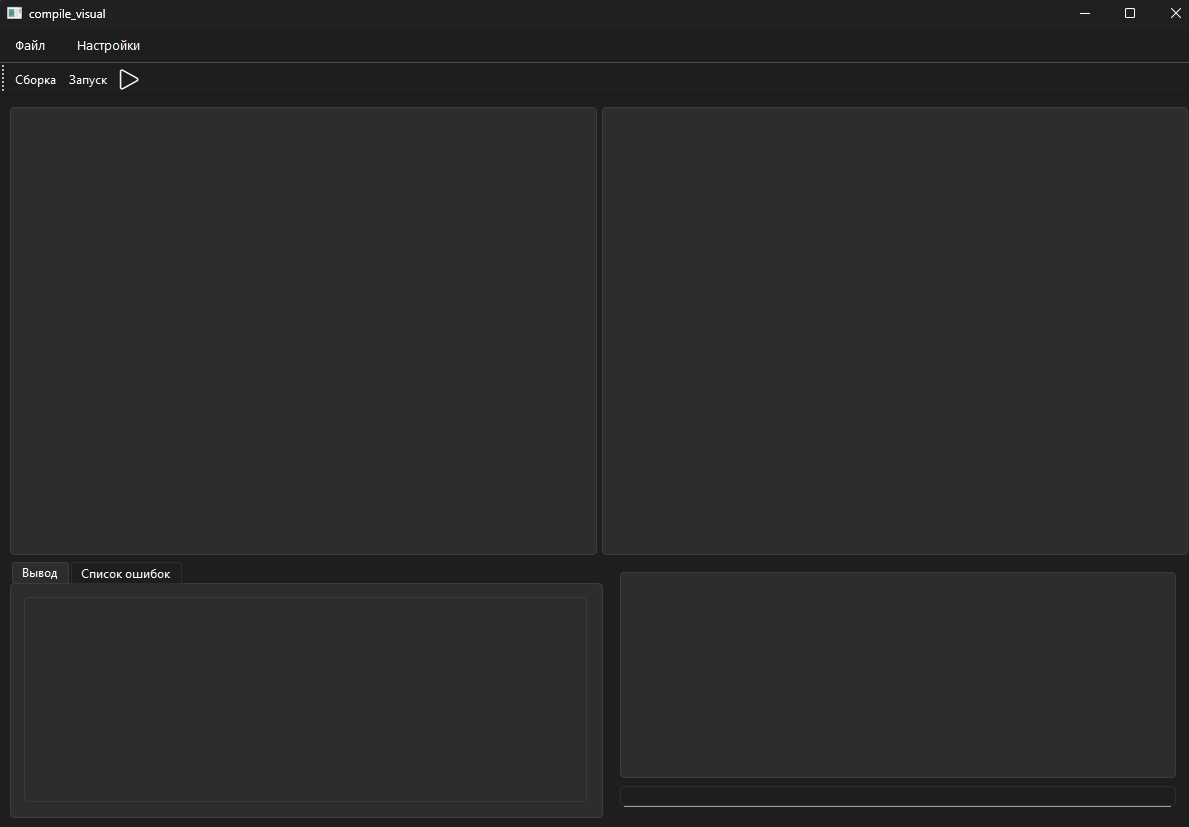
\includegraphics[width=0.75\linewidth]{image_2026-05-16_14-14-47.png}
    \caption{\centeringВизуальная среда разработки сразу после запуска}
    \label{fig:visual}
\end{figure}

Создание, открытие и сохранение файлов может выполняться пользователем через верхний набор меню <<Файл>>, а настройка автоподсветки лексем --- через меню <<Настройки>>. Иерархия меню <<Файл>> представлена на рисунках 8(a) - 8(c).
\begin{figure}[H]
    \centering
    % Первый рисунок
    \begin{subfigure}[b]{0.32\textwidth}
        \centering
        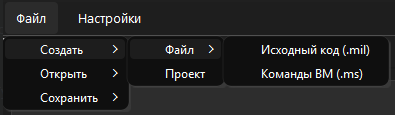
\includegraphics[width=1\linewidth]{image_file1.png}
        \caption{\centering Подменю <<Создать>>}
        \label{fig:sub1}
    \end{subfigure}
    \hfill % Равномерное распределение свободного пространства по горизонтали
    % Второй рисунок
    \begin{subfigure}[b]{0.32\textwidth}
        \centering
        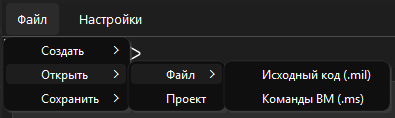
\includegraphics[width=1\linewidth]{image_file2.png}
        \caption{\centering Подменю <<Открыть>>}
        \label{fig:sub2}
    \end{subfigure}
    \hfill
    % Третий рисунок
    \begin{subfigure}[b]{0.32\textwidth}
        \centering
        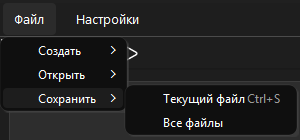
\includegraphics[width=1\linewidth]{image_file3.png}
        \caption{\centering Подменю <<Сохранить>>}
        \label{fig:sub3}
    \end{subfigure}
    
    \caption{\centering Иерархия меню <<Файл>>}
    \label{fig:file}
\end{figure}

После открытия файла, сборки программы и её запуска все текстовые окна заполняются выводами. На рисунке 9 изображена среда разработки после выполнения данных действий.

\begin{figure}[H]
    \centering
    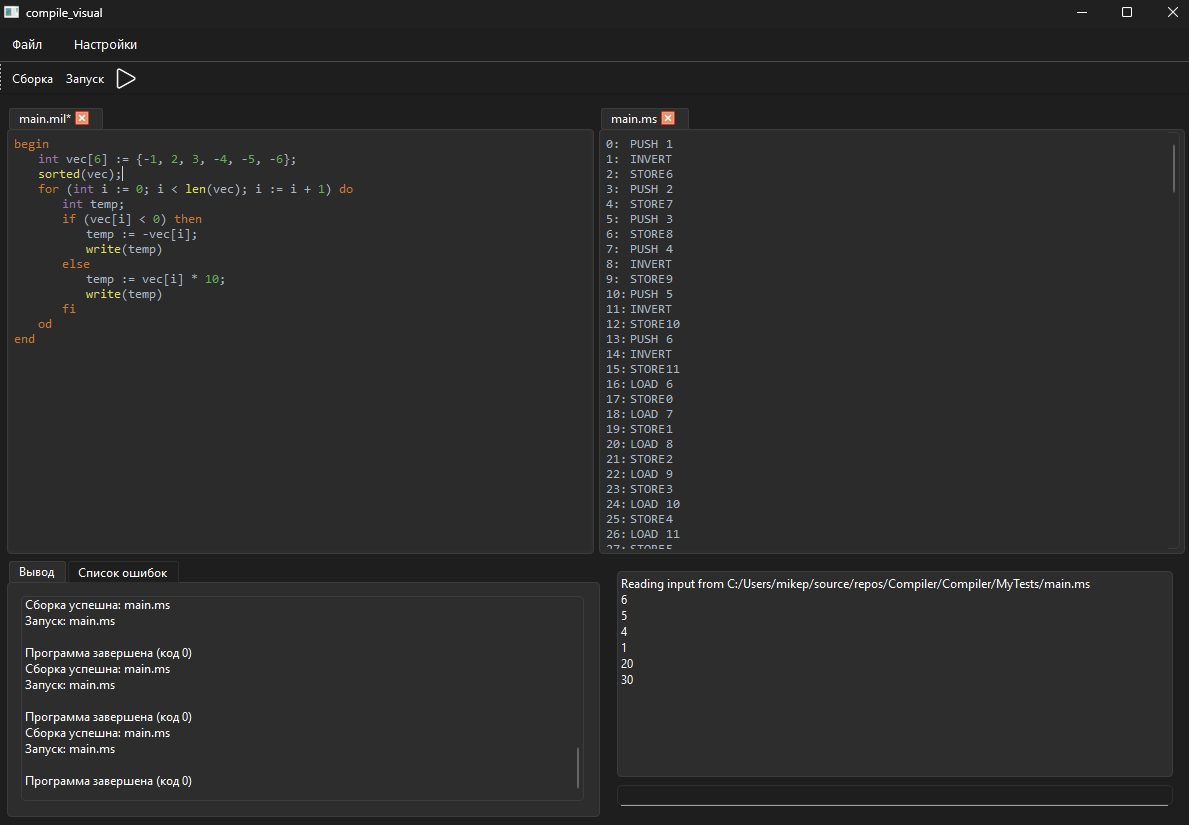
\includegraphics[width=0.75\linewidth]{image_build.png}
    \caption{\centeringВизуальная среда разработки после открытия файла, сборки и запуска программы}
    \label{build}
\end{figure}

Через секунду после остановки ввода текста пользователем в редактор исходного кода запускается лексический анализ, который позволяет создать подсветку лексем и ошибок. В случае обнаружения лексической ошибки, место её обнаружения подчеркивается красным цветом. Если во время компиляции программы были обнаружены такие ошибки, пишется соответствующее сообщение в вывод компиляции, при этом прошлый сгенерированный код остаётся доступен для запуска.

На рисунке 10 изображен вывод компиляции и подчеркивание ошибок при наличии в коде программы идентификаторов начинающихся с цифры и состоящих из символов кириллицы.

\begin{figure}[H]
    \centering
    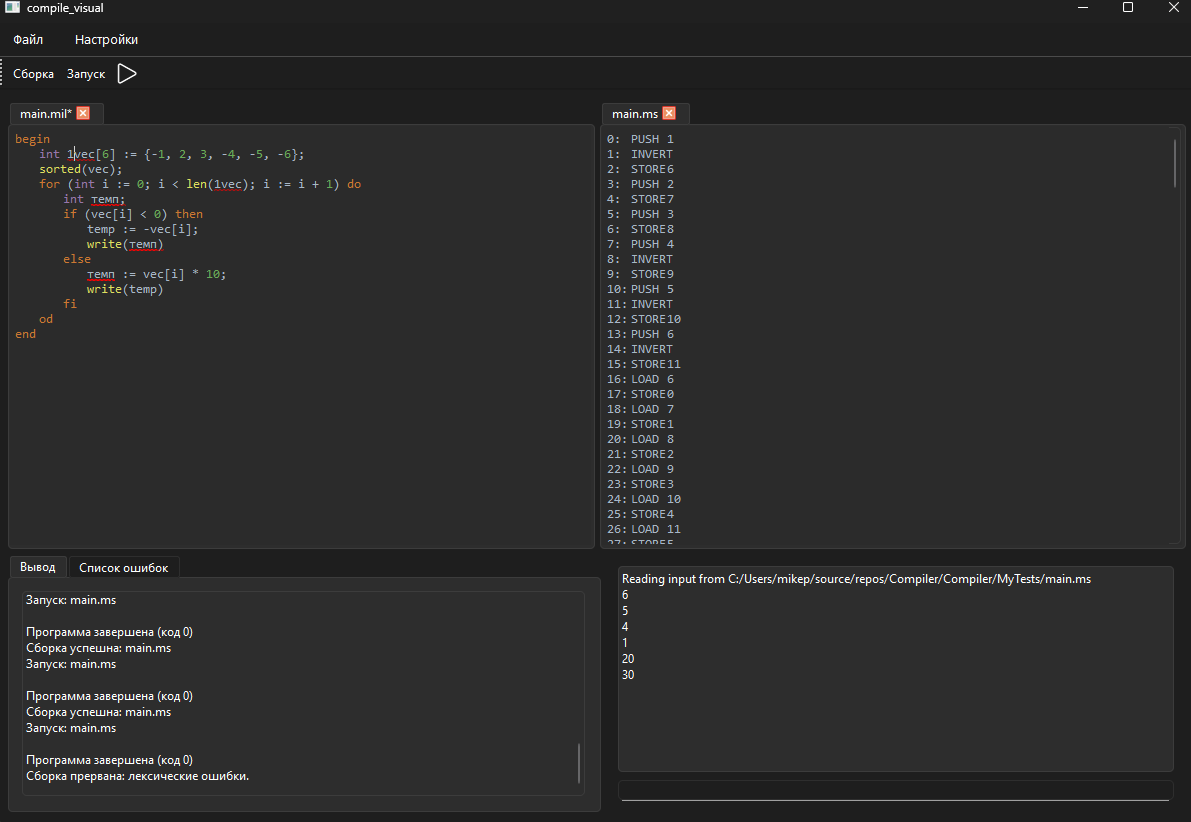
\includegraphics[width=0.75\linewidth]{image_errors.png}
    \caption{\centeringВизуальная среда разработки после сборки программы, содержащей лексические ошибки}
    \label{build}
\end{figure}

Также если во время компиляции программы во время синтаксического анализа обнаружены синтаксические ошибки, компиляция завершается и в её вывод пишутся сообщения об ошибках. На рисунке 11 представлен вывод компиляции при наличии необъявленного идентификатора и точки с запятой после последнего оператора в блоке.

\begin{figure}[H]
    \centering
    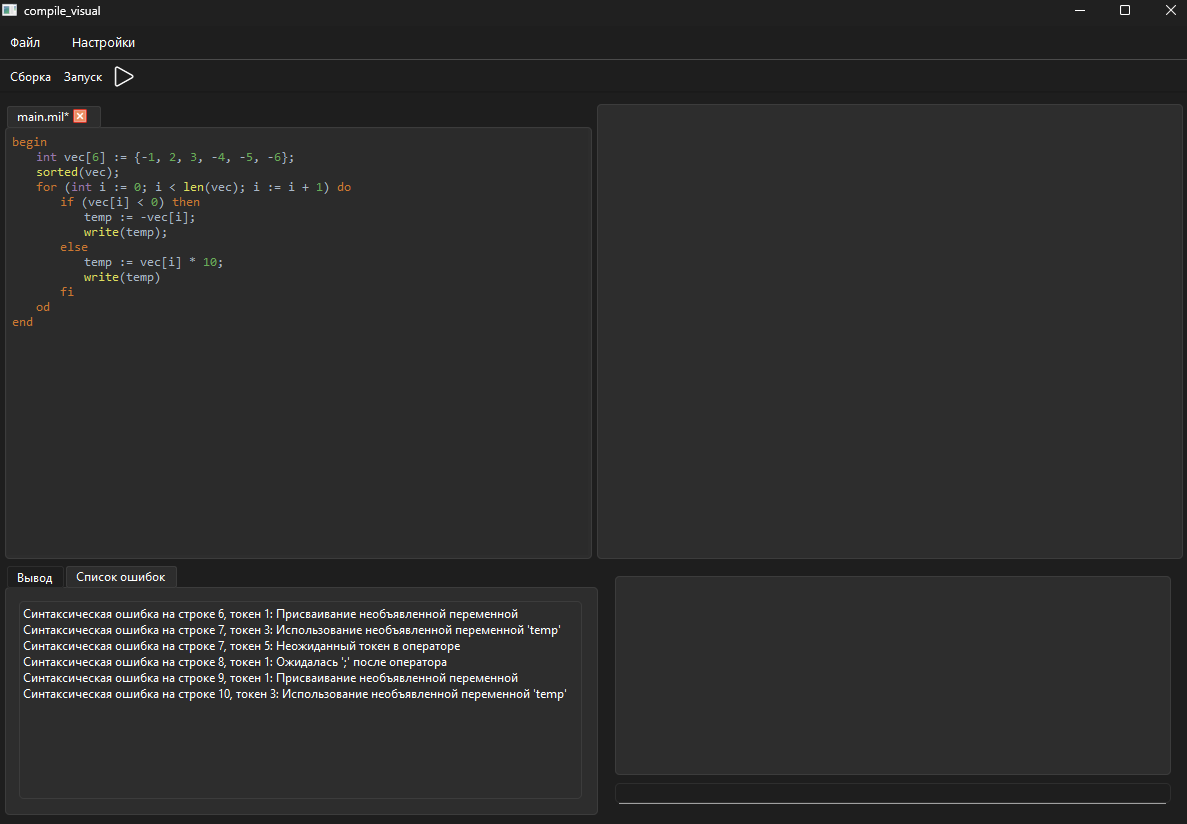
\includegraphics[width=0.75\linewidth]{image_sint_error.png}
    \caption{\centeringВизуальная среда разработки после сборки программы, содержащей синтаксические ошибки}
    \label{build}
\end{figure}

Среда разработки поддерживает работу сразу с несколькими файлами, при этом сценарии работы текущий файл для каждого окна можно перерключать с поомщью нажатия на соответствующую вкладку над редактором. При изменении файла к его названию во вкладке добавляется символ <<*>>, а при попытке выхода из программы с одним или несколькими несохранёнными файлами выводится диалог с предложением сохранения для каждого такого файла.

На рисунке 12 изображена попытка закрытия среды разработки при налии нескольких несохранённых файлов.

\begin{figure}[H]
    \centering
    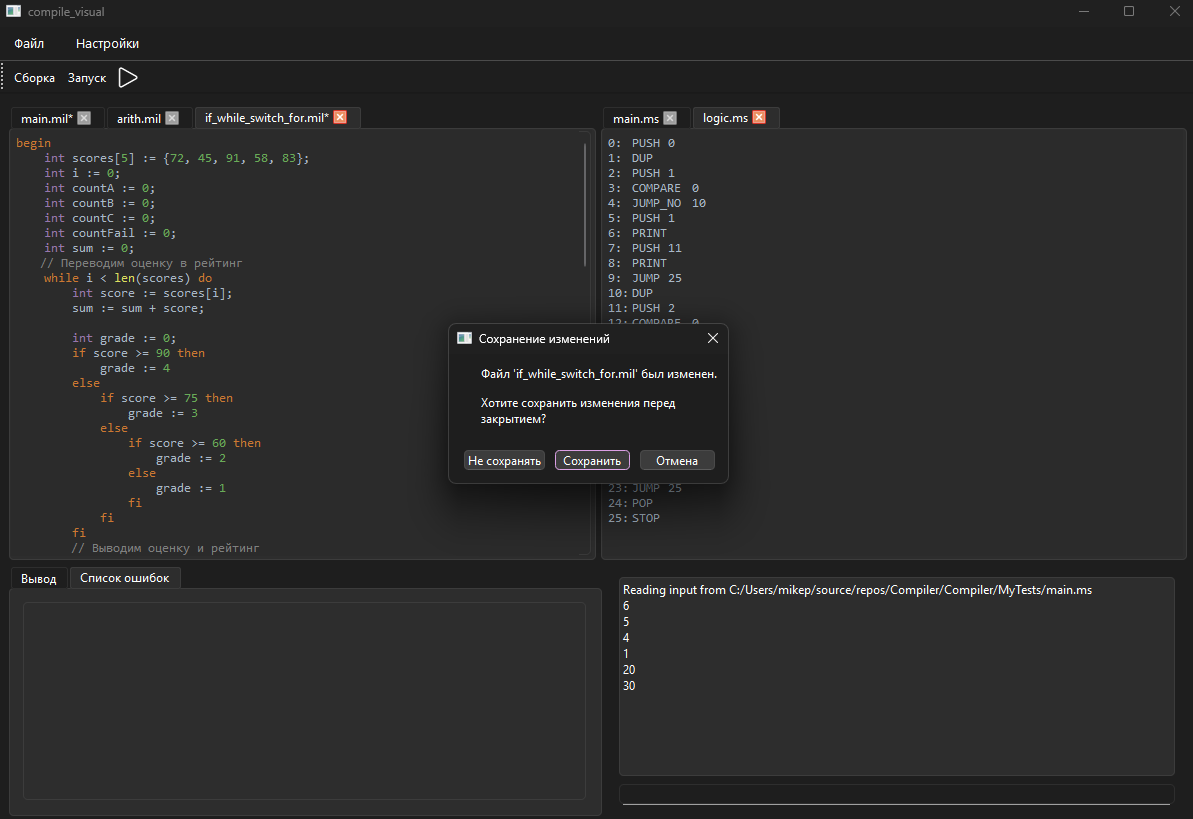
\includegraphics[width=0.75\linewidth]{image_unsaved.png}
    \caption{\centering Вывод диалога при закрытии программы с несохранёнными файлами}
    \label{build}
\end{figure}


\subsection{Стандартные операторы}
На листинге 17 отображен код программы содержащей базовые операторы языка MiLan, а на рисунке 13 представлен вывод этой программы.

\begin{lstlisting}[caption={Стандартные операторы}]
Begin
	int i := 0;
	while i < 10 do
		i := i + 1;
		if i > 5 then
			write(i)
		else
			write(-i)
		fi
	od
	
	
	
End
\end{lstlisting}

\begin{figure}[H]
    \centering
    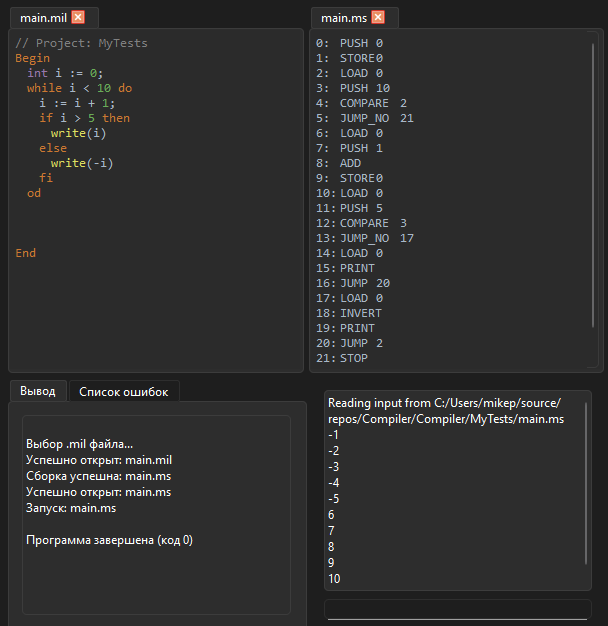
\includegraphics[width=0.75\linewidth]{image7.png}
    \caption{\centeringРезультат компиляции и запуска программы 1}
\end{figure}

\subsection{Цикл for}
На листинге 18 отображен код программы содержащей цикл for, а на рисунке 14 представлен вывод этой программы.

\begin{lstlisting}[caption={Цикл for}]
Begin
	for (int i := 0; i < 40; i := i + 3) do
		if i - (i / 2) * 2 = 1 then
			write (i)
		fi
	od
End
\end{lstlisting}

\begin{figure}[H]
    \centering
    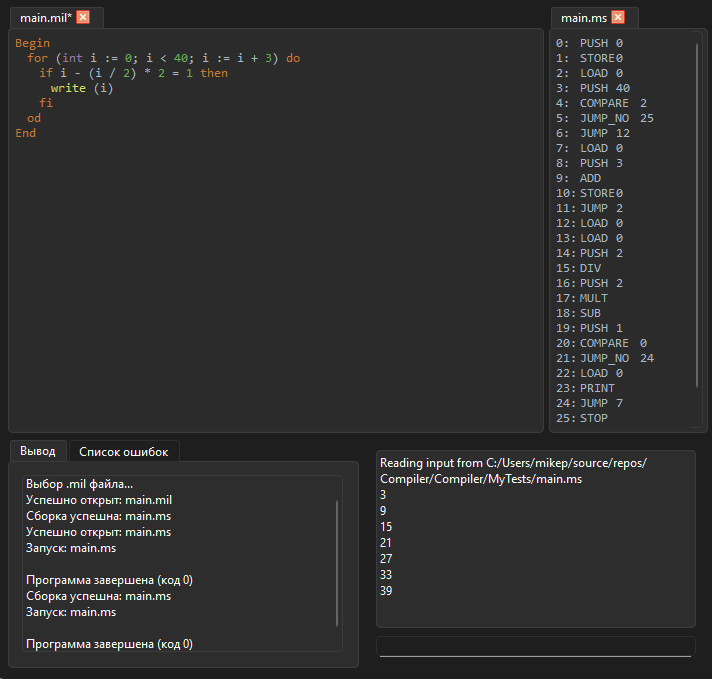
\includegraphics[width=0.75\linewidth]{image8.png}
    \caption{\centeringРезультат компиляции и запуска программы 2}
\end{figure}


\subsection{Булевы константы и операции над ними}
На листинге 19 представлен код программы содержащей булевы константы и операции над ними, а на рисунке 15 представлен вывод этой программы.

\begin{lstlisting}[caption={Булевы конcтанты и операции}]
begin
	int x := 5;
	int y := 10;
	bool a := x < y;
	bool b := x = y;
	bool c := x != y && y > 0;
	bool d := false || x > 3;
	write(a);
	write(b);
	write(c);
	write(d)
end
\end{lstlisting}

\begin{figure}[H]
    \centering
    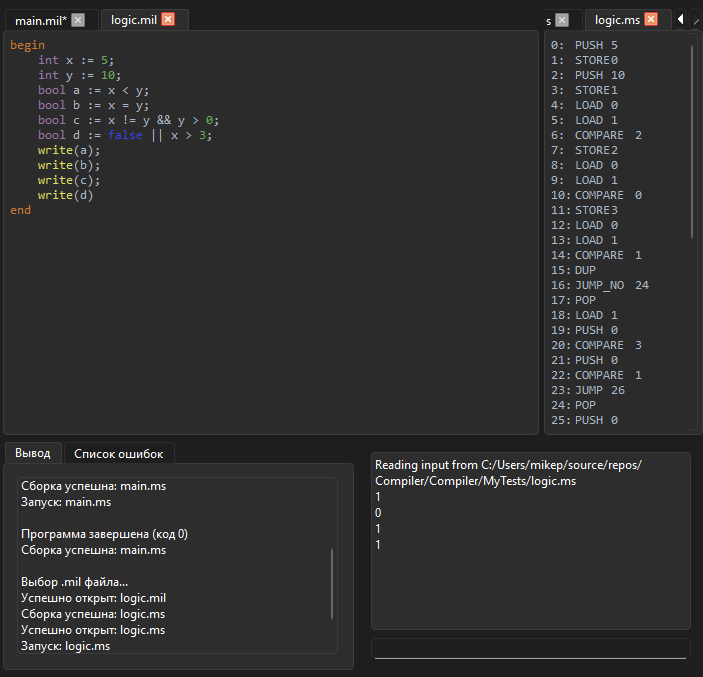
\includegraphics[width=0.75\linewidth]{image9.png}
    \caption{\centeringРезультат компиляции и запуска программы 3}
\end{figure}

\subsection{Одномерные массивы и операции над ними}
На листинге 20 представлен код программы содержащей одномерные массивы и операции над ними, а на рисунке 16 представлен вывод этой программы.
\begin{lstlisting}[caption={Одномерные массивы}]
begin
    	int arr[5] := {10, 20, 30, 40, 50};
    	write(arr[0:2]);
	fill(arr, 0);
	write(arr[0:2]);
	replace(arr, 0, 999);
	write(arr[0]);
	write(111111);
	write(resize(resize(arr, 2, 0), 5, -1))
    
end
\end{lstlisting}

\begin{figure}[H]
    \centering
    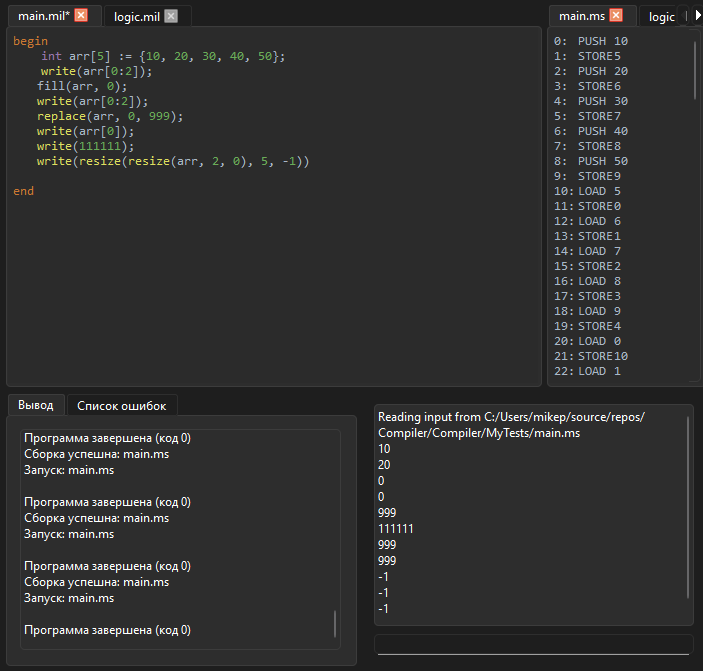
\includegraphics[width=0.75\linewidth]{image10.png}
    \caption{\centeringРезультаты компиляции и запуска программы 4}
\end{figure}

\subsection{Двумерные массивы и операции над ними}
На листинге 19 можно увидеть код программы содержащей двумерные массивы и операции над ними, а также умножение по правилам Шимбелла и комментарии.

На рисунке 17 представлен вывод этой программы.

\begin{lstlisting}[caption={Двумерные массивы, комментарии, Шимбелл}]
begin
	int a[2][2] := {{1, 0}, {2, 3}};
	int b[2][2] := {{7, 4}, {4, 1}};
	    
	int c[2][2];
	c := a * b;
	write(c);
	// Умножение по правилам Шимбелла
	write(shimb(a, c, 1));
	write(tovector(a))
	/* многострочный
	комментарий
	*/ 
end
\end{lstlisting}

\begin{figure}[H]
    \centering
    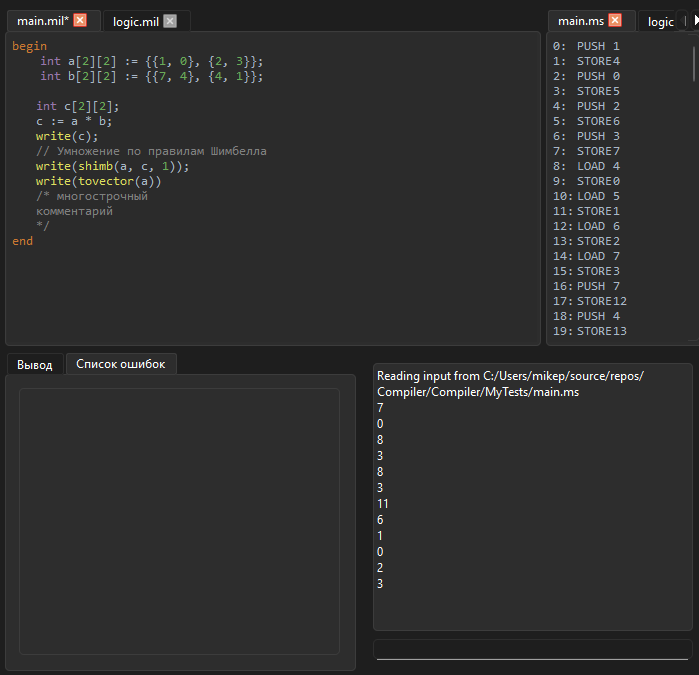
\includegraphics[width=0.75\linewidth]{image11.png}
    \caption{\centeringРезультаты компиляции и запуска программы 5}
\end{figure}

\subsection{Конструкция switch ... case}
На листинге 20 приведён код программы содержащей конструкцию sw, а также умножение по правилам Шимбелла и комментарии.

На рисунке 18 представлен вывод этой программы.

\begin{lstlisting}[caption={Конструкция switch ... case}]
    begin
    int i := 2;
		switch (i) begin
				case 1: write(1) break;
				case 2: write(2); write(2) break;
				case 3: write(3) break;
				case 4: write(4) break;
				default: write(-1)
		endcase
		int i := 90;
		switch (i) begin
				case 1: write(1) break;
				case 2: write(2) break;
				case 3: write(3) break;
				case 4: write(4) break;
				default: write(-1)
		endcase
end
\end{lstlisting}

\begin{figure}[H]
    \centering
    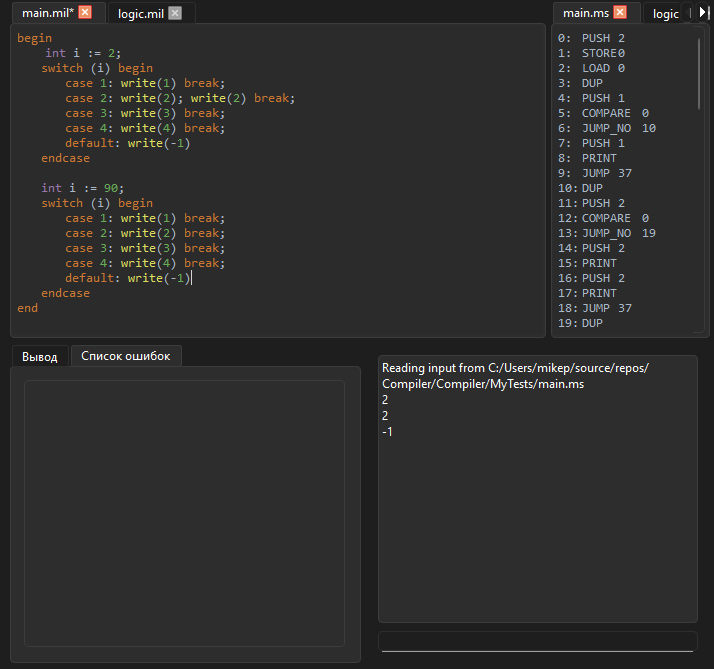
\includegraphics[width=0.75\linewidth]{image12.png}
    \caption{\centeringРезультаты компиляции и запуска программы 6}
\end{figure}

\newpage
\section*{Заключение}
\addcontentsline{toc}{section}{Заключение}
В ходе выполнения данной лабораторной работы были проанализированы существующие языки программирования C++, Ruby и JavaScript, а также изучена реализация операций, которыми необходимо было расширить язык программирования MiLan. Были реализованы следующие типы данных, конструкции, операторы:
\begin{itemize}
    \item Оператор выбора.
    \item Оператор цикла for.
    \item Булевы константы, переменные и операции на ними.
    \item Одномерные и двумерные массивы и операции над ними.
    \item Перемножение матриц по правилам Шимбелла и все виды комментариев.
    \item Арифметические поэлементные операции над одномерными и двумерными массивами.
\end{itemize}

Все операции над одномерными и двумерными массивами были реализованы как <<опасные>> методы из ЯП Ruby, что позволяет данным операторам и менять исходный объект массива и также возвращать изменённый объект (то есть операторы не являются ни мутирующими ни иммутабельными в классическом понимании). Данная реализация позволяет уменьшить размер исходного кода программы, но требует от программиста большей внимательности при написании кода.

Расширенная грамматика ЯП MiLan была записана в БНФ-нотации, а также для её правил были составлены синтаксические диаграммы.

Лексический анализатор для распознавания лексем в программе был реализован с помощью автомата, что обеспечивает высокую скорость лексического анализа и возможность использовать динамическую подсветку лексем в коде программы. 

Грамматика языка MiLan относится ко второму типу в иерархии Хомского (контекстно-свободная грамматика). Для синтаксического анализа был использован метод рекурсивного спуска. Данный метод реализует работу анализатора LL(1).

Достоинства реализации:
\begin{itemize}
    \item Использование конечного автомата при лексическом анализе обеспечивает высокую скорость определения лексем в тексте программы, что позволяет организовать автоматическую подсветку лексем, за минимальное время.
    \item Реализованная среда разработки позволяет более удобно редактировать код, так как в ней реализована подсветка лексем.
\end{itemize}

Недостатки реализации:
\begin{itemize}
    \item Одномерные и двумерные массивы реализованы только со статической памятью, что сильно ограничивает их использование в программах.
\end{itemize}

Масштабирование:
\begin{itemize}
    \item Добавить возможность создания переменных в динамической памяти и работы с указателями.
    \item Реализовать другие типы данных, например float и string.
    \item Добавить этап оптимизации.
\end{itemize}

\newpage
\addcontentsline{toc}{section}{Список использованной литературы}
\begin{thebibliography}{}
    \bibitem{litlink1} Секция <<Телематика>>.— Текст: электронный // tema.spbstu: [сайт].— URL: https://tema.spbstu.ru/mathem/ (дата обращения: 29.04.2026).
\end{thebibliography}

\newpage

\section*{Приложение A. Исходный код метода initTM}
\addcontentsline{toc}{section}{Приложение A. Исходный код метода initTM}
\footnotesize{
\begin{lstlisting}[language=C++]
inline FSM<std::wstring>* initTm(
	std::wstring& buffer,
	Group& currentGroup,
	std::vector<Lexem*>& lexemTable,
	std::vector<Error*>& errorTable,
	std::map<int, int>& lexemsR
) {
	FSM<std::wstring>::TransitionMap tM;
	FSM<std::wstring>* fsm = new FSM<std::wstring>();


	auto addToLexemsR = [&lexemsR]() {
		lexemsR.insert({ currentRow, currentLexem });
		currentLexem++;
		};


	auto y1 = [&fsm](wchar_t c) {fsm->popFront(); };
	auto y2 = [&buffer](wchar_t c) { buffer += c; };
	auto y3 = [&buffer](wchar_t c) { buffer.clear(); };
	auto y4 = [&buffer](wchar_t c) { currentRow++; currentPos = 1; };
	auto y_Div = [&lexemTable, &buffer, &addToLexemsR](wchar_t c) { lexemTable.push_back(&lDiv); addToLexemsR(); };
	auto y_Id = [&lexemTable, &buffer, &addToLexemsR](wchar_t c) { lexemTable.push_back(new Lexem(buffer, Id)); addToLexemsR(); };
	auto y_Plus = [&lexemTable, &buffer, &addToLexemsR](wchar_t c) { lexemTable.push_back(&lPlus); addToLexemsR(); };
	auto y_Diff = [&lexemTable, &buffer, &addToLexemsR](wchar_t c) { lexemTable.push_back(&lDiff); addToLexemsR(); };
	auto y_Mult = [&lexemTable, &buffer, &addToLexemsR](wchar_t c) { lexemTable.push_back(&lMult); addToLexemsR(); };
	auto y_LBracket = [&lexemTable, &buffer, &addToLexemsR](wchar_t c) { lexemTable.push_back(&lLBracket); addToLexemsR(); };
	auto y_RBracket = [&lexemTable, &buffer, &addToLexemsR](wchar_t c) { lexemTable.push_back(&lRBracket); addToLexemsR(); };
	auto y_LCurly = [&lexemTable, &buffer, &addToLexemsR](wchar_t c) { lexemTable.push_back(&lLCurly); addToLexemsR(); };
	auto y_RCurly = [&lexemTable, &buffer, &addToLexemsR](wchar_t c) { lexemTable.push_back(&lRCurly); addToLexemsR(); };
	auto y_LSquare = [&lexemTable, &buffer, &addToLexemsR](wchar_t c) { lexemTable.push_back(&lLSquare); addToLexemsR(); };
	auto y_RSquare = [&lexemTable, &buffer, &addToLexemsR](wchar_t c) { lexemTable.push_back(&lRSquare); addToLexemsR(); };
	auto y_Assign = [&lexemTable, &buffer, &addToLexemsR](wchar_t c) { lexemTable.push_back(&lAssign); addToLexemsR(); };
	auto y_Semicolon = [&lexemTable, &buffer, &addToLexemsR](wchar_t c) { lexemTable.push_back(&lSemicolon); addToLexemsR(); };
	auto y_Comma = [&lexemTable, &buffer, &addToLexemsR](wchar_t c) { lexemTable.push_back(&lComma); addToLexemsR(); };
	auto y_Var = [&lexemTable, &buffer, &addToLexemsR](wchar_t c) { lexemTable.push_back(new Lexem(buffer, Var)); addToLexemsR(); };
	auto y_ShortAnd = [&lexemTable, &buffer, &addToLexemsR](wchar_t c) { lexemTable.push_back(&lShortAnd); addToLexemsR(); };
	auto y_FullAnd = [&lexemTable, &buffer, &addToLexemsR](wchar_t c) { lexemTable.push_back(&lFullAnd); addToLexemsR(); };
	auto y_ShortOr = [&lexemTable, &buffer, &addToLexemsR](wchar_t c) { lexemTable.push_back(&lShortOr); addToLexemsR(); };
	auto y_FullOr = [&lexemTable, &buffer, &addToLexemsR](wchar_t c) { lexemTable.push_back(&lFullOr); addToLexemsR(); };
	auto y_Equal = [&lexemTable, &buffer, &addToLexemsR](wchar_t c) { lexemTable.push_back(&lEqual); addToLexemsR(); };
	auto y_NotEqual = [&lexemTable, &buffer, &addToLexemsR](wchar_t c) { lexemTable.push_back(&lNotEqual); addToLexemsR(); };
	auto y_Not = [&lexemTable, &buffer, &addToLexemsR](wchar_t c) { lexemTable.push_back(&lNot); addToLexemsR(); };
	auto y_LessEqual = [&lexemTable, &buffer, &addToLexemsR](wchar_t c) { lexemTable.push_back(&lLessEqual); addToLexemsR(); };
	auto y_Less = [&lexemTable, &buffer, &addToLexemsR](wchar_t c) { lexemTable.push_back(&lLess); addToLexemsR(); };
	auto y_GreaterEqual = [&lexemTable, &buffer, &addToLexemsR](wchar_t c) { lexemTable.push_back(&lGreaterEqual); addToLexemsR(); };
	auto y_Greater = [&lexemTable, &buffer, &addToLexemsR](wchar_t c) { lexemTable.push_back(&lGreater); addToLexemsR(); };
	auto y_Begin = [&lexemTable, &buffer, &addToLexemsR](wchar_t c) { lexemTable.push_back(&lBegin); addToLexemsR(); };
	auto y_Break = [&lexemTable, &buffer, &addToLexemsR](wchar_t c) { lexemTable.push_back(&lBreak); addToLexemsR(); };
	auto y_Bool = [&lexemTable, &buffer, &addToLexemsR](wchar_t c) { lexemTable.push_back(&lBool); addToLexemsR(); };
	auto y_Case = [&lexemTable, &buffer, &addToLexemsR](wchar_t c) { lexemTable.push_back(&lCase); addToLexemsR(); };
	auto y_Continue = [&lexemTable, &buffer, &addToLexemsR](wchar_t c) { lexemTable.push_back(&lContinue); addToLexemsR(); };
	auto y_Do = [&lexemTable, &buffer, &addToLexemsR](wchar_t c) { lexemTable.push_back(&lDo); addToLexemsR(); };
	auto y_End = [&lexemTable, &buffer, &addToLexemsR](wchar_t c) { lexemTable.push_back(&lEnd); addToLexemsR(); };
	auto y_Else = [&lexemTable, &buffer, &addToLexemsR](wchar_t c) { lexemTable.push_back(&lElse); addToLexemsR(); };
	auto y_For = [&lexemTable, &buffer, &addToLexemsR](wchar_t c) { lexemTable.push_back(&lFor); addToLexemsR(); };
	auto y_False = [&lexemTable, &buffer, &addToLexemsR](wchar_t c) { lexemTable.push_back(&lFalse); addToLexemsR(); };
	auto y_Find = [&lexemTable, &buffer, &addToLexemsR](wchar_t c) { lexemTable.push_back(&lFind); addToLexemsR(); };
	auto y_Fi = [&lexemTable, &buffer, &addToLexemsR](wchar_t c) { lexemTable.push_back(&lFi); addToLexemsR(); };
	auto y_Int = [&lexemTable, &buffer, &addToLexemsR](wchar_t c) { lexemTable.push_back(&lInt); addToLexemsR(); };
	auto y_If = [&lexemTable, &buffer, &addToLexemsR](wchar_t c) { lexemTable.push_back(&lIf); addToLexemsR(); };
	auto y_Len = [&lexemTable, &buffer, &addToLexemsR](wchar_t c) { lexemTable.push_back(&lLen); addToLexemsR(); };
	auto y_Od = [&lexemTable, &buffer, &addToLexemsR](wchar_t c) { lexemTable.push_back(&lOd); addToLexemsR(); };
	auto y_Replace = [&lexemTable, &buffer, &addToLexemsR](wchar_t c) { lexemTable.push_back(&lReplace); addToLexemsR(); };
	auto y_Reverse = [&lexemTable, &buffer, &addToLexemsR](wchar_t c) { lexemTable.push_back(&lReverse); addToLexemsR(); };
	auto y_Resize = [&lexemTable, &buffer, &addToLexemsR](wchar_t c) { lexemTable.push_back(&lResize); addToLexemsR(); };
	auto y_Read = [&lexemTable, &buffer, &addToLexemsR](wchar_t c) { lexemTable.push_back(&lRead); addToLexemsR(); };
	auto y_Switch = [&lexemTable, &buffer, &addToLexemsR](wchar_t c) { lexemTable.push_back(&lSwitch); addToLexemsR(); };
	auto y_Shimb = [&lexemTable, &buffer, &addToLexemsR](wchar_t c) { lexemTable.push_back(&lShimb); addToLexemsR(); };
	auto y_True = [&lexemTable, &buffer, &addToLexemsR](wchar_t c) { lexemTable.push_back(&lTrue); addToLexemsR(); };
	auto y_Then = [&lexemTable, &buffer, &addToLexemsR](wchar_t c) { lexemTable.push_back(&lThen); addToLexemsR(); };
	auto y_While = [&lexemTable, &buffer, &addToLexemsR](wchar_t c) { lexemTable.push_back(&lWhile); addToLexemsR(); };
	auto y_Write = [&lexemTable, &buffer, &addToLexemsR](wchar_t c) { lexemTable.push_back(&lWrite); addToLexemsR(); };
	auto y_Trans = [&lexemTable, &buffer, &addToLexemsR](wchar_t c) { lexemTable.push_back(&lTrans); addToLexemsR(); };

	auto y_Colon = [&lexemTable, &buffer, &addToLexemsR](wchar_t c) { lexemTable.push_back(&lColon); addToLexemsR(); };
	auto y_ToVector = [&lexemTable, &buffer, &addToLexemsR](wchar_t c) { lexemTable.push_back(&lToVector); addToLexemsR(); };
	auto y_Default = [&lexemTable, &buffer, &addToLexemsR](wchar_t c) { lexemTable.push_back(&lDefault); addToLexemsR(); };
	auto y_Sorted = [&lexemTable, &buffer, &addToLexemsR](wchar_t c) { lexemTable.push_back(&lSorted); addToLexemsR(); };
	auto y_Comment = [&lexemTable, &buffer, &addToLexemsR](wchar_t c) { lexemTable.push_back(new Lexem(buffer, Comment)); };
	auto y_MultiComment = [&lexemTable, &buffer, &addToLexemsR](wchar_t c) { lexemTable.push_back(new Lexem(buffer, MultiComment)); };

	auto y_Fill = [&lexemTable, &buffer, &addToLexemsR](wchar_t c) { lexemTable.push_back(&lFill); addToLexemsR(); };
	auto y_Copy = [&lexemTable, &buffer, &addToLexemsR](wchar_t c) { lexemTable.push_back(&lCopy); addToLexemsR(); };
	auto y_EndCase = [&lexemTable, &buffer, &addToLexemsR](wchar_t c) { lexemTable.push_back(&lEndCase); addToLexemsR(); };

	auto y_GroupNone = [&currentGroup](wchar_t c) { currentGroup = gNone; };
	auto y_GroupComment = [&currentGroup](wchar_t c) { currentGroup = gComment; };
	auto y_GroupMultiComment = [&currentGroup](wchar_t c) { currentGroup = gMultiComment; };
	auto y_GroupId = [&currentGroup](wchar_t c) { currentGroup = gId; };
	auto y_GroupVar = [&currentGroup](wchar_t c) { currentGroup = gVar; };
	auto y_GroupWord = [&currentGroup](wchar_t c) { currentGroup = gWord; };


	tM[0] = {
		{1, {is_ws, {y1}}},
		{2, {[](wchar_t c) {return c == L'/'; } , {y2, y1}}},
		{15, {[](wchar_t c) {return c == L'+'; } , {y_Plus, y1}}},
		{16, {[](wchar_t c) {return c == L'-'; } , {y_Diff, y1}}},
		{17, {[](wchar_t c) {return c == L'*'; } , {y_Mult, y1}}},
		{18, {[](wchar_t c) {return c == L'('; } , {y_LBracket, y1}}},
		{19, {[](wchar_t c) {return c == L')'; } , {y_RBracket, y1}}},
		{20, {[](wchar_t c) {return c == L'{'; } , {y_LCurly, y1}}},
		{21, {[](wchar_t c) {return c == L'}'; } , {y_RCurly, y1}}},
		{22, {[](wchar_t c) {return c == L'['; } , {y_LSquare, y1}}},
		{23, {[](wchar_t c) {return c == L']'; } , {y_RSquare, y1}}},
		{24, {[](wchar_t c) {return c == L':'; } , {y2, y1}}},
		{26, {[](wchar_t c) {return c == L';'; } , {y_Semicolon, y1}}},
		{27, {[](wchar_t c) {return c == L','; } , {y_Comma, y1}}},
		{28, {is_digit, {y_GroupVar, y2, y1}}},
		{36, {[](wchar_t c) {return c == L'&'; } , {y2, y1}}},
		{39, {[](wchar_t c) {return c == L'|'; } , {y2, y1}}},
		{42, {[](wchar_t c) {return c == L'='; } , {y_Equal, y1}}},
		{43, {[](wchar_t c) {return c == L'!'; } , {y2, y1}}},
		{45, {[](wchar_t c) {return c == L'<'; } , {y2, y1}}},
		{48, {[](wchar_t c) {return c == L'>'; } , {y2, y1}}},
		{51, {[](wchar_t c) {return tl(c) == L'b'; } , {y_GroupWord, y2, y1}}},
		{60, {[](wchar_t c) {return tl(c) == L'c'; } , {y_GroupWord, y2, y1}}},
		{71, {[](wchar_t c) {return tl(c) == L'd'; } , {y_GroupWord, y2, y1}}},
		{73, {[](wchar_t c) {return tl(c) == L'e'; } , {y_GroupWord, y2, y1}}},
		{79, {[](wchar_t c) {return tl(c) == L'f'; } , {y_GroupWord, y2, y1}}},
		{94, {[](wchar_t c) {return tl(c) == L'i'; } , {y_GroupWord, y2, y1}}},
		{98, {[](wchar_t c) {return tl(c) == L'l'; } , {y_GroupWord, y2, y1}}},
		{101, {[](wchar_t c) {return tl(c) == L'o'; } , {y_GroupWord, y2, y1}}},
		{103, {[](wchar_t c) {return tl(c) == L'r'; } , {y_GroupWord, y2, y1}}},
		{125, {[](wchar_t c) {return tl(c) == L's'; } , {y_GroupWord, y2, y1}}},
		{140, {[](wchar_t c) {return tl(c) == L't'; } , {y_GroupWord, y2, y1}}},
		{147, {[](wchar_t c) {return tl(c) == L'w'; } , {y_GroupWord, y2, y1}}},
		{12, {[](wchar_t c) {return is_letter(tl(c)); }, {y_GroupId, y2, y1}}},
	};

	tM[1] = {
		{0, {ret_true, {y_GroupNone}}}
	};
	tM[2] = {
		{3, {[](wchar_t c) {return c == L'/'; } , {y_GroupComment, y2, y1}}},
		{6, {[](wchar_t c) {return c != L'/' && c != L'*'; } , {y_Div, y3}}},
		{7, {[](wchar_t c) {return c == L'*'; } , {y_GroupMultiComment, y2, y1}}}
	};
	tM[3] = {
		{4, {[](wchar_t c) {return c != L'\n'; } , {y2, y1}}},
		{5, {[](wchar_t c) {return c == L'\n'; } , {y4, y_Comment, y3, y1}}}
	};
	tM[4] = {
		{4, {[](wchar_t c) {return c != L'\n'; } , {y2, y1}}},
		{5, {[](wchar_t c) {return c == L'\n'; } , {y4, y_Comment, y3, y1}}}
	};
	tM[5] = {
		{0, {ret_true, {y_GroupNone}}}
	};
	tM[6] = {
		{0, {ret_true, {y_GroupNone}}}
	};
	tM[7] = {
		{8, {[](wchar_t c) {return c == L'\n'; } , {y4, y2, y1}}},
		{8, {[](wchar_t c) {return c != L'*'; } , {y2, y1}}},
		{9, {[](wchar_t c) {return c == L'*'; } , {y2, y1}}}
	};
	tM[8] = {
		{8, {[](wchar_t c) {return c == L'\n'; } , {y4, y2, y1}}},
		{8, {[](wchar_t c) {return c != L'*'; } , {y2, y1}}},
		{9, {[](wchar_t c) {return c == L'*'; } , {y2, y1}}}
	};
	tM[9] = {
		{10, {[](wchar_t c) {return c == L'/'; } , {y2, y_MultiComment, y3, y1}}},
		{11, {[](wchar_t c) {return c == L'\n'; } , {y4, y2, y1}}},
		{11, {[](wchar_t c) {return is_ws(c) or c != L'/'; } , {y2, y1}}}
	};
	tM[10] = {
		{0, {ret_true, {y_GroupNone}}}
	};
	tM[11] = {
		{8, {[](wchar_t c) {return c == L'\n'; } , {y4, y2, y1}}},
		{8, {[](wchar_t c) {return c != L'*'; } , {y2, y1}}},
		{9, {[](wchar_t c) {return c == L'*'; } , {y2, y1}}}
	};
	tM[12] = {
		{13, {[](wchar_t c) {return not (is_digit(c) or is_letter(tl(c))); } , {y_Id, y3}}},
		{14, {[](wchar_t c) {return is_digit(c) or is_letter(tl(c)); } , {y2, y1}}}
	};
	tM[13] = {
		{0, {ret_true, {y_GroupNone}}}
	};
	tM[14] = {
		{13, {[](wchar_t c) {return not (is_digit(c) or is_letter(tl(c))); } , {y_Id, y3}}},
		{14, {[](wchar_t c) {return is_digit(c) or is_letter(tl(c)); } , {y2, y1}}}
	};
	tM[15] = {
		{0, {ret_true, {y_GroupNone}}}
	};
	tM[16] = {
		{0, {ret_true, {y_GroupNone}}}
	};
	tM[17] = {
		{0, {ret_true, {y_GroupNone}}}
	};
	tM[18] = {
		{0, {ret_true, {y_GroupNone}}}
	};
	tM[19] = {
		{0, {ret_true, {y_GroupNone}}}
	};
	tM[20] = {
		{0, {ret_true, {y_GroupNone}}}
	};
	tM[21] = {
		{0, {ret_true, {y_GroupNone}}}
	};
	tM[22] = {
		{0, {ret_true, {y_GroupNone}}}
	};
	tM[23] = {
		{0, {ret_true, {y_GroupNone}}}
	};
	tM[24] = {
		{25, {[](wchar_t c) {return c == L'='; }, {y_Assign, y3, y1}}},
		{157, {[](wchar_t c) {return c != L'='; }, {y_Colon, y3}}}
	};
	tM[25] = {
		{0, {ret_true, {y_GroupNone}}}
	};
	tM[26] = {
		{0, {ret_true, {y_GroupNone}}}
	};
	tM[27] = {
		{0, {ret_true, {y_GroupNone}}}
	};
	tM[28] = {
		{28, {is_digit, {y2, y1}}},
		{29, {[](wchar_t c) {return not is_digit(c) and not is_letter(tl(c)); }, {y_Var, y3}}}
	};
	tM[29] = {
		{0, {ret_true, {y_GroupNone}}}
	};
	tM[36] = {
		{37, {[](wchar_t c) {return c == L'&'; }, {y_ShortAnd, y3, y1}}},
		{38, {[](wchar_t c) {return c != L'&'; }, {y_FullAnd, y3}}}
	};
	tM[37] = {
		{0, {ret_true, {y_GroupNone}}}
	};
	tM[38] = {
		{0, {ret_true, {y_GroupNone}}}
	};
	tM[39] = {
		{40, {[](wchar_t c) {return c == L'|'; }, {y_ShortOr, y3, y1}}},
		{41, {[](wchar_t c) {return c != L'|'; }, {y_FullOr, y3}}}
	};
	tM[40] = {
		{0, {ret_true, {y_GroupNone}}}
	};
	tM[41] = {
		{0, {ret_true, {y_GroupNone}}}
	};
	tM[42] = {
		{0, {ret_true, {y_GroupNone}}}
	};
	tM[43] = {
		{44, {[](wchar_t c) {return c == L'='; }, {y_NotEqual, y3, y1}}},
		{156, {[](wchar_t c) {return c != L'='; }, {y_Not, y3}}}
	};
	tM[44] = {
		{0, {ret_true, {y_GroupNone}}}
	};
	tM[156] = {
		{0, {ret_true, {y_GroupNone}}}
	};
	tM[45] = {
		{46, {[](wchar_t c) {return c == L'='; }, {y_LessEqual, y3, y1}}},
		{47, {[](wchar_t c) {return c != L'='; }, {y_Less, y3}}}
	};
	tM[46] = {
		{0, {ret_true, {y_GroupNone}}}
	};
	tM[47] = {
		{0, {ret_true, {y_GroupNone}}}
	};
	tM[48] = {
		{49, {[](wchar_t c) {return c == L'='; }, {y_GreaterEqual, y3, y1}}},
		{50, {[](wchar_t c) {return c != L'='; }, {y_Greater, y3}}}
	};
	tM[49] = {
		{0, {ret_true, {y_GroupNone}}}
	};
	tM[50] = {
		{0, {ret_true, {y_GroupNone}}}
	};
	tM[51] = {
		{52, {[](wchar_t c) {return tl(c) == L'e'; }, {y2, y1}} },
		{56, {[](wchar_t c) {return tl(c) == L'r'; }, {y2, y1}} },
		{82, {[](wchar_t c) {return tl(c) == L'o'; }, {y2, y1}} }
	};
	tM[52] = {
		{53, {[](wchar_t c) {return tl(c) == L'g'; }, {y2, y1}} }
	};
	tM[53] = {
		{54, {[](wchar_t c) {return tl(c) == L'i'; }, {y2, y1}} }
	};
	tM[54] = {
		{55, {[](wchar_t c) {return tl(c) == L'n'; }, {y_Begin, y3, y1}} }
	};
	tM[55] = {
		{0, {ret_true, {}} }
	};
	tM[56] = {
		{57, {[](wchar_t c) {return tl(c) == L'e'; }, {y2, y1}} }
	};
	tM[57] = {
		{58, {[](wchar_t c) {return tl(c) == L'a'; }, {y2, y1}} }
	};
	tM[58] = {
		{59, {[](wchar_t c) {return tl(c) == L'k'; }, {y_Break, y3, y1}} }
	};
	tM[59] = {
		{0, {ret_true, {}} }
	};
	tM[60] = {
		{61, {[](wchar_t c) {return tl(c) == L'a'; }, {y2, y1}} },
		{64, {[](wchar_t c) {return tl(c) == L'o'; }, {y2, y1}} }
	};
	tM[61] = {
		{62, {[](wchar_t c) {return tl(c) == L's'; }, {y2, y1}} }
	};
	tM[62] = {
		{63, {[](wchar_t c) {return tl(c) == L'e'; }, {y_Case, y3, y1}} }
	};
	tM[63] = {
		{0, {ret_true, {}} }
	};
	tM[64] = {
		{65, {[](wchar_t c) {return tl(c) == L'n'; }, {y2, y1}} },
		{32, {[](wchar_t c) {return tl(c) == L'p'; }, {y2, y1}}}
	};
	tM[32] = {
		{33, {[](wchar_t c) {return tl(c) == L'y'; }, {y_Copy, y3, y1}}}
	};
	tM[33] = {
		{0, {ret_true, {}} }
	};
	tM[65] = {
		{66, {[](wchar_t c) {return tl(c) == L't'; }, {y2, y1}} }
	};
	tM[66] = {
		{67, {[](wchar_t c) {return tl(c) == L'i'; }, {y2, y1}} }
	};
	tM[67] = {
		{68, {[](wchar_t c) {return tl(c) == L'n'; }, {y2, y1}} }
	};
	tM[68] = {
		{69, {[](wchar_t c) {return tl(c) == L'u'; }, {y2, y1}} }
	};
	tM[69] = {
		{70, {[](wchar_t c) {return tl(c) == L'e'; }, {y_Continue, y3, y1}} }
	};
	tM[70] = {
		{0, {ret_true, {}} }
	};
	tM[71] = {
		{72, {[](wchar_t c) {return tl(c) == L'o'; }, {y_Do, y3, y1}} },
		{158, {[](wchar_t c) {return tl(c) == L'e'; }, {y2, y1}}}
	};
	tM[72] = {
		{0, {ret_true, {}} }
	};
	tM[73] = {
		{74, {[](wchar_t c) {return tl(c) == L'n'; }, {y2, y1}} },
		{76, {[](wchar_t c) {return tl(c) == L'l'; }, {y2, y1}} }
	};
	tM[74] = {
		{75, {[](wchar_t c) {return tl(c) == L'd'; }, {y1}} }
	};
	tM[75] = {
		{179, {[](wchar_t c) {return tl(c) == L'c'; }, {y2, y1}} },
		{0, {ret_true, {y_End, y3}} }
	};
	tM[179] = {
		{180, {[](wchar_t c) {return tl(c) == L'a'; }, {y2, y1}} },
	};
	tM[180] = {
		{181, {[](wchar_t c) {return tl(c) == L's'; }, {y2, y1}} },
	};
	tM[181] = {
		{182, {[](wchar_t c) {return tl(c) == L'e'; }, {y_EndCase, y3, y1}} },
	};
	tM[182] = {
		{0, {ret_true, {}} }
	};
	tM[76] = {
		{77, {[](wchar_t c) {return tl(c) == L's'; }, {y2, y1}} }
	};
	tM[77] = {
		{78, {[](wchar_t c) {return tl(c) == L'e'; }, {y_Else, y3, y1}} }
	};
	tM[78] = {
		{0, {ret_true, {}} }
	};
	tM[79] = {
		{80, {[](wchar_t c) {return tl(c) == L'o'; }, {y2, y1}} },
		{86, {[](wchar_t c) {return tl(c) == L'a'; }, {y2, y1}} },
		{90, {[](wchar_t c) {return tl(c) == L'i'; }, {y2, y1}} }
	};
	tM[80] = {
		{81, {[](wchar_t c) {return tl(c) == L'r'; }, {y_For, y3, y1}} }
	};
	tM[81] = {
		{0, {ret_true, {}} }
	};
	tM[86] = {
		{87, {[](wchar_t c) {return tl(c) == L'l'; }, {y2, y1}} }
	};
	tM[87] = {
		{88, {[](wchar_t c) {return tl(c) == L's'; }, {y2, y1}} }
	};
	tM[88] = {
		{89, {[](wchar_t c) {return tl(c) == L'e'; }, {y_False, y3, y1}} }
	};
	tM[89] = {
		{0, {ret_true, {}} }
	};
	tM[90] = {
		{91, {[](wchar_t c) {return tl(c) == L'n'; }, {y2, y1}} },
		{93, {[](wchar_t c) {return not(is_digit(c) or is_letter(tl(c))); }, {y_Fi, y3}} },
		{30, {[](wchar_t c) {return tl(c) == L'l'; }, {y2, y1}}}
	};
	tM[30] = {
		{31, {[](wchar_t c) {return tl(c) == L'l'; }, {y_Fill, y3, y1}}}
	};
	tM[31] = {
		{0, {ret_true, {}} }
	};
	tM[91] = {
		{92, {[](wchar_t c) {return tl(c) == L'd'; }, {y_Find, y3, y1}} }
	};
	tM[92] = {
		{0, {ret_true, {}} }
	};
	tM[93] = {
		{0, {ret_true, {}} }
	};
	tM[94] = {
		{95, {[](wchar_t c) {return tl(c) == L'n'; }, {y2, y1}} },
		{97, {[](wchar_t c) {return tl(c) == L'f'; }, {y_If, y3, y1}} }
	};
	tM[95] = {
		{96, {[](wchar_t c) {return tl(c) == L't'; }, {y_Int, y3, y1}} }
	};
	tM[96] = {
		{0, {ret_true, {}} }
	};
	tM[97] = {
		{0, {ret_true, {}} }
	};
	tM[98] = {
		{99, {[](wchar_t c) {return tl(c) == L'e'; }, {y2, y1}} },
	};
	tM[99] = {
		{100, {[](wchar_t c) {return tl(c) == L'n'; }, {y_Len, y3, y1}} }
	};
	tM[100] = {
		{0, {ret_true, {}} }
	};
	tM[101] = {
		{102, {[](wchar_t c) {return tl(c) == L'd'; }, {y_Od, y3, y1}} },
	};
	tM[102] = {
		{0, {ret_true, {}} }
	};
	tM[103] = {
		{104, {[](wchar_t c) {return tl(c) == L'e'; }, {y2, y1}} },
	};
	tM[104] = {
		{105, {[](wchar_t c) {return tl(c) == L'p'; }, {y2, y1}} },
		{110, {[](wchar_t c) {return tl(c) == L'v'; }, {y2, y1}} },
		{115, {[](wchar_t c) {return tl(c) == L's'; }, {y2, y1}} },
		{119, {[](wchar_t c) {return tl(c) == L'a'; }, {y2, y1}} }
	};
	tM[105] = {
		{106, {[](wchar_t c) {return tl(c) == L'l'; }, {y2, y1}} }
	};
	tM[106] = {
		{107, {[](wchar_t c) {return tl(c) == L'a'; }, {y2, y1}} }
	};
	tM[107] = {
		{108, {[](wchar_t c) {return tl(c) == L'c'; }, {y2, y1}} }
	};
	tM[108] = {
		{109, {[](wchar_t c) {return tl(c) == L'e'; }, {y_Replace, y3, y1}} }
	};
	tM[109] = {
		{0, {ret_true, {}} }
	};
	tM[110] = {
		{111, {[](wchar_t c) {return tl(c) == L'e'; }, {y2, y1}} }
	};
	tM[111] = {
		{112, {[](wchar_t c) {return tl(c) == L'r'; }, {y2, y1}} }
	};
	tM[112] = {
		{113, {[](wchar_t c) {return tl(c) == L's'; }, {y2, y1}} }
	};
	tM[113] = {
		{114, {[](wchar_t c) {return tl(c) == L'e'; }, {y_Reverse, y3, y1}} }
	};
	tM[114] = {
		{0, {ret_true, {}} }
	};
	tM[115] = {
		{116, {[](wchar_t c) {return tl(c) == L'i'; }, {y2, y1}} }
	};
	tM[116] = {
		{117, {[](wchar_t c) {return tl(c) == L'z'; }, {y2, y1}} }
	};
	tM[117] = {
		{118, {[](wchar_t c) {return tl(c) == L'e'; }, {y_Resize, y3, y1}} }
	};
	tM[118] = {
		{0, {ret_true, {}} }
	};
	tM[119] = {
		{120, {[](wchar_t c) {return tl(c) == L'd'; }, {y_Read, y3, y1}} }
	};
	tM[120] = {
		{0, {ret_true, {}} }
	};
	tM[125] = {
		{131, {[](wchar_t c) {return tl(c) == L'w'; }, {y2, y1}} },
		{136, {[](wchar_t c) {return tl(c) == L'h'; }, {y2, y1}} },
		{164, {[](wchar_t c) {return tl(c) == L'o'; }, {y2, y1}} }
	};
	tM[131] = {
		{132, {[](wchar_t c) {return tl(c) == L'i'; }, {y2, y1}} }
	};
	tM[132] = {
		{133, {[](wchar_t c) {return tl(c) == L't'; }, {y2, y1}} }
	};
	tM[133] = {
		{134, {[](wchar_t c) {return tl(c) == L'c'; }, {y2, y1}} }
	};
	tM[134] = {
		{135, {[](wchar_t c) {return tl(c) == L'h'; }, {y_Switch, y3, y1}} }
	};
	tM[135] = {
		{0, {ret_true, {}} }
	};
	tM[136] = {
		{137, {[](wchar_t c) {return tl(c) == L'i'; }, {y2, y1}} }
	};
	tM[137] = {
		{138, {[](wchar_t c) {return tl(c) == L'm'; }, {y2, y1}} }
	};
	tM[138] = {
		{139, {[](wchar_t c) {return tl(c) == L'b'; }, {y_Shimb, y3, y1}} }
	};
	true;
	tM[139] = {
		{0, {ret_true, {}} }
	};
	tM[140] = {
		{141, {[](wchar_t c) {return tl(c) == L'r'; }, {y2, y1}} },
		{144, {[](wchar_t c) {return tl(c) == L'h'; }, {y2, y1}} },
		{169, {[](wchar_t c) {return tl(c) == L'o'; }, {y2, y1}} }
	};
	tM[141] = {
		{142, {[](wchar_t c) {return tl(c) == L'u'; }, {y2, y1}} },
		{176, {[](wchar_t c) {return tl(c) == L'a'; }, {y2, y1}} }
	};
	tM[142] = {
		{143, {[](wchar_t c) {return tl(c) == L'e'; }, {y_True, y3, y1}} }
	};
	tM[143] = {
		{0, {ret_true, {}} }
	};
	tM[144] = {
		{145, {[](wchar_t c) {return tl(c) == L'e'; }, {y2, y1}} }
	};
	tM[145] = {
		{146, {[](wchar_t c) {return tl(c) == L'n'; }, {y_Then, y3, y1}} }
	};
	tM[146] = {
		{0, {ret_true, {}} }
	};
	tM[147] = {
		{148, {[](wchar_t c) {return tl(c) == L'h'; }, {y2, y1}} },
		{152, {[](wchar_t c) {return tl(c) == L'r'; }, {y2, y1}} }
	};
	tM[148] = {
		{149, {[](wchar_t c) {return tl(c) == L'i'; }, {y2, y1}} }
	};
	tM[149] = {
		{150, {[](wchar_t c) {return tl(c) == L'l'; }, {y2, y1}} }
	};
	tM[150] = {
		{151, {[](wchar_t c) {return tl(c) == L'e'; }, {y_While, y3, y1}} }
	};
	tM[151] = {
		{0, {ret_true, {}} }
	};
	tM[152] = {
		{153, {[](wchar_t c) {return tl(c) == L'i'; }, {y2, y1}} }
	};
	tM[153] = {
		{154, {[](wchar_t c) {return tl(c) == L't'; }, {y2, y1}} }
	};
	tM[154] = {
		{155, {[](wchar_t c) {return tl(c) == L'e'; }, {y_Write, y3, y1}} }
	};
	tM[155] = {
		{0, {ret_true, {}} }
	};
	tM[156] = {
		{0, {ret_true, {y_GroupNone}}}
	};
	tM[157] = {
		{0, {ret_true, {y_GroupNone}}}
	};
	tM[158] = {
		{159, {[](wchar_t c) {return tl(c) == L'f'; }, {y2, y1}}}
	};
	tM[159] = {
		{160, {[](wchar_t c) {return tl(c) == L'a'; }, {y2, y1}}}
	};
	tM[160] = {
		{161, {[](wchar_t c) {return tl(c) == L'u'; }, {y2, y1}}}
	};
	tM[161] = {
		{162, {[](wchar_t c) {return tl(c) == L'l'; }, {y2, y1}}}
	};
	tM[162] = {
		{163, {[](wchar_t c) {return tl(c) == L't'; }, {y_Default, y3, y1}}}
	};
	tM[163] = {
		{0, {ret_true, {y_GroupNone}}}
	};
	tM[164] = {
		{165, {[](wchar_t c) {return tl(c) == L'r'; }, {y2, y1}}}
	};
	tM[165] = {
		{166, {[](wchar_t c) {return tl(c) == L't'; }, {y2, y1}}}
	};
	tM[166] = {
		{167, {[](wchar_t c) {return tl(c) == L'e'; }, {y2, y1}}}
	};
	tM[167] = {
		{168, {[](wchar_t c) {return tl(c) == L'd'; }, {y_Sorted, y3, y1}}}
	};
	tM[168] = {
		{0, {ret_true, {y_GroupNone}}}
	};
	tM[169] = {
		{170, {[](wchar_t c) {return tl(c) == L'v'; }, {y2, y1}}}
	};
	tM[170] = {
		{171, {[](wchar_t c) {return tl(c) == L'e'; }, {y2, y1}}}
	};
	tM[171] = {
		{172, {[](wchar_t c) {return tl(c) == L'c'; }, {y2, y1}}}
	};
	tM[172] = {
		{173, {[](wchar_t c) {return tl(c) == L't'; }, {y2, y1}}}
	};
	tM[173] = {
		{174, {[](wchar_t c) {return tl(c) == L'o'; }, {y2, y1}}}
	};
	tM[174] = {
		{175, {[](wchar_t c) {return tl(c) == L'r'; }, {y_ToVector, y3, y1}}}
	};
	tM[175] = {
		{0, {ret_true, {y_GroupNone}}}
	};
	tM[176] = {
		{177, {[](wchar_t c) {return tl(c) == L'n'; }, {y2, y1}}}
	};
	tM[177] = {
		{178, {[](wchar_t c) {return tl(c) == L'n'; }, {y_Trans, y3, y1}}}
	};
	tM[178] = {
		{0, {ret_true, {}} }
	};
	tM[82] = {
		{83, {[](wchar_t c) {return tl(c) == L'o'; }, {y2, y1}} }
	};
	tM[83] = {
		{84, {[](wchar_t c) {return tl(c) == L'l'; }, {y_Bool, y3, y1}} }
	};
	tM[84] = {
		{0, {ret_true, {}} }
	};

	auto errorProcessor = [&buffer, &currentGroup, &fsm, &errorTable, &lexemTable, &y_Comment, &addToLexemsR](bool isEnd) {
		int pos_delta = 0;
		int buffer_len = buffer.size();
		if (isEnd) {
			if (buffer_len != 0) {
				switch (currentGroup) {
				case gComment:
					lexemTable.push_back(new Lexem(buffer, Comment));
					buffer.clear();
					break;
				case gMultiComment:
					errorTable.push_back(new Error(currentRow, currentPos, buffer, L"Multirow comment is not finished"));
					buffer.clear();
					break;
				case gVar:
					errorTable.push_back(new Error(currentRow, currentPos, buffer, L"Value of Var is not finished"));
					buffer.clear();
					break;
				}
			}
			else {
				switch (currentGroup) {
				case gComment:
					y_Comment(L' ');
					buffer.clear();
					break;
				case gMultiComment:
					errorTable.push_back(new Error(currentRow, currentPos, buffer, L"Multirow comment is not finished"));
					buffer.clear();
					break;
				}
			}
		}
		else {
			switch (currentGroup) {
			case gNone:
				errorTable.push_back(new Error(currentRow, currentPos - 1, buffer, L"Unexpected symbol"));
				fsm->popFront();

				buffer.clear();
				fsm->setState(0);
				break;
			case gComment:
				errorTable.push_back(new Error(currentRow, currentPos, L"", L"Comment is not finished"));
				fsm->setState(0);
				break;
			case gId:
				errorTable.push_back(new Error(currentRow, currentPos, buffer, L"Unexpected symbol in identificator"));
				buffer.clear();
				fsm->setState(0);
				break;
			case gVar:
				errorTable.push_back(new Error(currentRow, currentPos, buffer, L"Unexpected symbol in variable"));
				while (is_digit(fsm->front()) or is_letter(fsm->front())) {
					buffer.push_back(fsm->front());
					fsm->popFront();
					pos_delta++;
				}
				buffer.clear();


				fsm->setState(0);
				break;
			case gWord:
				currentGroup = gId;
				fsm->setState(12);
				break;
			};
		}
		};

	fsm->assignTransitions(200, tM, errorProcessor);
	return fsm;
}
\end{lstlisting}
\end{document}